\documentclass[12pt,twoside]{report}
\usepackage[a4paper,width=150mm,top=25mm,bottom=25mm]{geometry}
\usepackage[cp1250]{inputenc}
\usepackage[czech]{babel}
\usepackage[IL2]{fontenc}
\usepackage{graphicx}
\usepackage{hyperref}
\hypersetup{
    colorlinks,
    citecolor=black,
    filecolor=black,
    linkcolor=black,
    urlcolor=black
}
\graphicspath{ {images/} }
\usepackage[nottoc,notlot,notlof]{tocbibind}
\usepackage{fancyhdr}
\pagestyle{fancy}
\fancyhead{}
\fancyhead[RO,LE]{Thesis Title}
\fancyfoot{}
\fancyfoot[LE,RO]{\thepage}
\fancyfoot[LO,CE]{Chapter \thechapter}
\fancyfoot[CO,RE]{Author Name}

\begin{document}

\tableofcontents

\chapter{�vod}
Tato pr�ce se zab�v� svobodn�m softwarem VuFind. Tento software poskytuje slu�bu rozhran� OPAC. P�vodn� byl vyv�jen pro kompatibilitu se softwarem Voyager, v~sou�asn� dob� je provozov�n i nad dal��mi softwary, kter� respektuj� form�t MARC21. Diplomov� pr�ce zpracov�v� technick� aspekty implementace a nasazen� tohoto syst�mu v~konkr�tn�m prost�ed�. Zdrojem informac� pro tuto pr�ci je p�ev�n� ofici�ln� dokumentace tohoto projektu \cite{vufind.oficial} a zku�enosti N�rodn� technick� knihovny (d�le jen NTK), kde je tento syst�m implementov�n. V n�sleduj�c� kapitole je p�edstavena filozofie svobodn�ho softwaru v�etn� n�kolika typick�ch p�edstavitel� z oblasti knihovnick�ch softwar�. Dal�� kapitola pojedn�v� o syst�mu VuFind; o jeho vzniku, kl��ov�ch vlastnostech, hardwarov�ch a softwarov�ch po�adavc�ch. Zm�n�na jsou specifika implementace NTK. Z�v�rem t�to kapitoly jsou uvedeny p��klady pou��v�n� VuFindu v tuzemsk�ch i zahrani�n�ch knihovn�ch. Ve �tvrt� kapitole jsou pops�ny technick� aspekty implementace port�lu VuFind se zam��en� na prost�ed� NTK; jsou vysv�tleny n�kter� konfigura�n� soubory, d�le autentikace u�ivatel�, proces importu a indexov�n� dat, specifika vyhled�v�n�, u�ivatelsk� modul, grafick� design a �ten��sk� konto. P�t� kapitola poskytuje informace o integraci syst�mu VuFind s knihovn�m syst�mem Aleph, o p�enosu dat mezi t�mito syst�my d�ky API rozhran� a o automatick�m skl�zen� dat p�es protokol OAI-PMH. V �est� kapitole je uvedeno konkr�tn� nasazen� port�lu VuFind v NTK, v�etn� popisu instalace i doty�n�ch server�, jak produk�n�ch, tak testovac�ch a experiment�ln�ch. Z�v�r t�to kapitoly je v�nov�n spr�v� provozu server� VuFind. V sedm� kapitole je nast�n�n mo�n� budouc� v�voj syst�mu VuFind.
\section{Historie NTK}
\label{sec:historientk}N�rodn� technick� knihovna je nejv�t�� a nejstar�� knihovnou technick� literatury v �esk� republice s kapacitou p�es 1,5 milionu svazk� \cite{techlib}. S p�est�hov�n�m z Mari�nsk�ho n�m�st� v are�lu Klementina na Star�m m�st� v Praze 1 do are�lu V� v Praze 6 - Dejvice v roce 2009 opustila i p�edchoz� n�zev St�tn� technick� knihovna \cite{stk}. Prim�rn� funkc� knihovny je poskytov�n� odborn�ch informa�n�ch slu�eb a zdroj� jak ti�t�n�ch tak elektronick�ch. Na d�lku poskytuje NTK elektronickou cestou kolem 18 tis�c odborn�ch �asopis� z oblasti techniky, p��rodn�ch v�d a medic�ny. Z�kazn�ci maj� p��stup i do vybran�ch on-line datab�z� a dal��ch elektronick�ch zdroj�. Sou��st� fondu NTK je tak� NU�L (N�rodn� �lo�i�t� �ed� literatury) \cite{techlib}.
Prvn� verze rozhran� VuFind v N�rodn� technick� knihovn� byla instalov�na na po��tku roku 2011 pod veden�m Ing. Milana Jan��ka. Jednalo se o v�vojovou verzi 1.1, kter� b�hem zhruba dvoulet�ho testov�n� a lad�n� pracovn�m t�mem NTK (Mgr. Jind�ich Mynarz byl posl�ze nahrazen Bc. Danielem Mare�kem) p�e�la do verze 1.3. Tato verze p�izp�soben� m�stn�m podm�nk�m byla ve zku�ebn�m provozu zhruba rok a od po��tku roku 2014 se stala hlavn�m vyhled�v�c�m rozhran�m ve�ejn�ho online katalogu N�rodn� technick� knihovny. V l�t� roku 2015 jedno�lenn� pracovn� t�m (Daniel Mare�ek) pod superviz� Mgr. Jana Kol�tora a ve spolupr�ci s extern�m grafick�m designerem upgradoval syst�m na zcela novou v�vojovou �adu 2, konkr�tn� verzi 2.3.1 spole�n� s jednotnou vizu�ln� prezentac� koresponduj�c� s webem knihovny.
\section{O VuFindu (p�edstaven� syst�mu)}
\label{sec:ovufindu}
V reakci na nedostatky tradi�n�ch knihovnick�ch OAPC� byl na p�d� americk� univerzitn� knihovny Villanova University's Falvey Memorial Library ve st�t� Pensylv�nie spu�t�n v�voj knihovnick�ho port�lu VuFind. N�zev tohoto syst�mu se proto skl�d� z akronymu n�zvu univerzity "Vu" (Villanova university) a anglick�ho slova "Find" (�esky hledat). Tento port�l je navr�en� a vyv�jen� knihovnami pro knihovny za ��elem umo�nit jejich u�ivatel�m vyhled�vat a proch�zet v�echny mo�n� zdroje, kter�mi dan� knihovna disponuje. Jeho prvn� verze 1.0 spat�ila sv�tlo sv�ta v �ervenci roku 2010\cite{prvni.verze}.

VuFind je pln� modul�rn�, co� znamen�, �e je mo�n� implementovat samostatn� pouze z�kladn� j�dro syst�mu s b�nou funkcionalitou, i z�rove� nadstavbov� komponenty, kter� funkcionalitu celkov�ho syst�mu zna�n� roz�i�uj�. D�ky tomu, �e tento port�l pat�� mezi svobodn� softwary, je mo�n� upravovat i p�id�vat jednotliv� moduly dle po�adavk� konkr�tn� knihovny a doc�lit tak maxim�ln�ho komfortu. Krom� toho, d�ky �irok� �k�le konfigura�n�ch mo�nost� je mo�n� syst�m rozs�hle customizovat bez nutnosti m�nit zdrojov� k�d.

Vyhled�vac�m j�drem VuFindu je Solr. Tato platforma, Apache Solr, je produktem neziskov� organizace Apache Software Foundation, kter� produkuje, podporuje a vyv�j� v�ce ne� 350 projekt� svobodn�ho software\cite{http://www.apache.org/}. Solr je open source software napsan� v programovac�m jazyce Java a nab�z� ��asn� v�kon a �k�lovatelnost, d�ky �emu� se odezvy na vyhled�vac� dotazy pohybuj� v ��dech milisekund. Je-li pot�eba rozlo�it zat�en� katalogu na v�ce server�, uplatn� se jeho schopnost distribuovanosti.

VuFind je poskytov�n zcela zdarma pod licenc� pro svobodn� software GNU General Public License. To znamen� jeho voln� u��v�n�, upravov�n� a sd�len� v r�mci jakkoliv r�znorod�ch knihovnick�ch komunit, co� posiluje a roz�i�uje mo�nosti tohoto syst�mu. Celkov� tento projekt povzbuzuje myslitele, hackery a profesion�ln� program�tory, aby navrhovali, upravovali, zlep�ovali a p�isp�vali do VuFindu a dal��ch open source softwar� s c�lem vytvo�it �ivotaschopn� �e�en� pro knihovny v�ech velikost�.
!about!


Kl��ov� vlastnosti vlastnosti
Fasetov� vyhled�v�n�.
VuFind umo��uje u�ivateli vyhled�vat skrz jednoduch� jedno��dkov� vyhled�vac� pole a d�le upravovat mno�inu v�sledk� pouh�m klik�n�m na polo�ky �azen� do faset. Lze t�m mno�inu v�sledk� zmen�ovat t�m zp�sobem, �e se v�sledky bu� omez� na zvolenou volbu, nebo naopak zvolen� volba se z v�sledk� vylou��. V r�mci n�kter�ch faset lze hesla kombinovat, jin� fasety umo��uj� vybrat pouze jednu hodnotu. To z�le�� na konkr�tn�m nastaven�, kter� lze samoz�ejm� m�nit dle pot�eby.
Status dostupnosti.
U ka�d�ho z�znamu ve v�sledc�ch vyhled�v�n� se zobrazuje status dostupnosti dan�ho titulu. D�ky technologii AJAX se tato informace z�sk�v� dotazov�n�m katalogu v re�ln�m �ase a d�je se tak nepozorovan� bez jak�hokoliv zpomalov�n� na��t�n� str�nky.
Podobn� jednotky.
V n�hledu z�znamu se zobrazuje nab�dka n�kolika podobn�ch titul�, co� u�ivateli pom�h� p�i v�b�ru a v orientaci v dan�m oboru.
U�ivatelsk� seznamy.
U�ivatel m� mo�nost ukl�dat jak cel� v�sledky vyhled�v�n�, tak jednotliv� z�znamy do vlastn�ch u�ivatelsky editovateln�ch seznam�. Seznamy jsou v syst�mu ulo�eny trvale, mohou b�t tedy zobrazeny kdykoliv. Tato vlastnost pom�h� u�ivateli organizovat svoji bibliografii a z�rove� d�ky sv� jednoduchosti odstra�uje nutnost pou��v�n� desktopov�ch, �asto p��li� slo�it�ch, cita�n�ch mana�er�.
Proch�zen� zdroj�.
U�ivatel m� mo�nost proch�zet v�echny zdroje, kter� knihovna nab�z�. Nen� tak omezen pouze na v�sledky vyhled�v�n�, kter� zobrazuj� jen ur�itou ��st fondu.
Biografie autor�.
D�ky mo�nosti napojit do VuFindu extern� zdroje jako je nap�.: Wikipedie, jsou u�ivateli zobrazeny informace o autorovi. U�ivatel tak z�sk� roz�i�uj�c� kontext, co� pom�h� k utvo�en� souvislost� k dan�mu d�lu.
Trval� URL.
Str�nky ve VuFindu, a� u� s v�sledky vyhled�v�n� nebo se samotn�mi z�znamy, jsou identifikov�ny trval�mi URL, d�ky �emu� si u�ivatel m��e p�idat str�nku mezi obl�ben� ve sv�m internetov�m prohl�e�i a m� tak na ur�it� m�sto st�l� p��stup.
Cita�n� mana�ery.
Kompatibilita se Zotero...
Internacionalizace.
Webov� rozhran� VuFindu je mo�n� p�ep�nat do p�eklad� sv�tov�ch jazyk� jako jsou brazilsk� portugal�tina, ��n�tina, holand�tina, angli�tina, francouz�tina, n�m�ina, japon�tina, �pan�l�tina a dal��ch. Tak� je mo�n� jednoduch�m zp�sobem vytvo�it p�eklad vlastn�.
P��stup k dat�m.
VuFind m� mnoho rozhran� pro programov�n� aplikac� (API). P�en�en� dat mezi institucemi lze pomoc� OAI protokolu. Vyhled�vac� algoritmus VuFindu je mo�n� vyu��t tak� OpenSearch zp�sobem. A pro p��stup k indexovan�m dat�m slou�� rozhran� vyhled�vac�ho a indexa�n�ho n�stroje Solr.


\cite{vufind.org}

zajimava firma nabizi implementaci open source library sw - koha, evergreen, vufind,..
https://www.ptfs-europe.com/customers/

Specifikace, requirements,..
Solr, hardware, linux, windows, Apache, Tom Cat,..
V��et software
NTK takov� po�adavky samoz�ejm� spl�uje a nav�c pou��v� je�t� dal�� souvisej�c� software...


\chapter{(Virtu�ln�) prost�ed� NTK}
\label{sec:chapter02}
V N�rodn� technick� knihovn� je servrovna, kde b�� lok�ln� virtu�ln� servery. Na jednom z nich b�� testovac� verze VuFindu. Zde prob�h� v�voj syst�mu. Na dal��m serveru, v�konn�j��m, b�� produk�n� verze VuFindu. Zat�mco produk�n� server je samoz�ejm� dostupn� z vn�j��ho prost�ed� knihovny v s�ti internet, testovac� verze je p��stupn� pouze z po��ta�� uvnit� instituce. 
\section{Hardware}
\label{sec:hwntk}
Servery - Aleph, SFX, Redmine, VuFind1, VuFind2, VuFind.test, VuFind-eiz.test
\section{Software}
\label{sec:swntk}
Software nutny pro VuFind - obecne

OS - moznosti(+vysvetlit obecne) + co pouzivame v knihovne(+ popis konkretniho)
web server - moznosti(+vysvetlit obecne) + co pouzivame v knihovne(+ popis konkretniho)
java server - moznosti(+vysvetlit obecne) + co pouzivame v knihovne(+ popis konkretniho)
...

OS
Apache - Http server
Jetty - Java servlet
zabezpe�en� - firewall

shibboleth
ssh

git, cron, sledovac� server Zabbix - presunout do provozu?


obrazky do jine kapitoly- architektura celeho vufindu - nakreslit - sablonovaci system navazuje na Controller - v podstate ZendFramework - MVC system
obrazek modulu mozna
obrazky(asi jeden) harvestovani, import, indexace :))


\chapter{VuFind v NTK}
\label{sec:chapter03}
N�rodn� technick� knihovna m� zhruba 27 000 registrovan�ch z�kazn�k�, pro kter� je ve VuFindu vytvo�eno u�ivatelsk� konto. Knihovn� fond obsahuje zhruba 1 200 000 jednotek, jejich� z�znamy jsou indexov�ny ve VuFindu a po�et v�p�j�ek z knihovn�ho fondu za jeden rok je zhruba 200 000, jejich� po�adavky p�ich�zej� od u�ivatel� z VuFindu. V takov�chto n�roc�ch prost�ed� N�rodn� technick� knihovny VuFind obst�l a proto mohl b�t vybr�n jako hlavn� vyhled�vac� port�l knihovny pro fyzick� fond. \cite{vyrocni.zprava}

Jedn�m z d�vod� pro nasazen� svobodn�ho softwaru VuFind v N�rodn� technick� knihovn� byl fakt, �e pro doposud pou��van� OPAC Aleph nebylo zakoupeno testovac� prost�ed� a tedy v�voj tohoto webov�ho rozhran� mohl prob�hat pouze v produk�n� verzi b�hem provozu, co� nen� zcela p�ijateln� pro z�kazn�ky syst�mu. 

S nemo�nost� vyv�jet syst�m a dr�et tak krok s p��chodem nov�ch technologi�
 
K nahrazen� dosavadn�ho OPACu p�isp�l i fakt,�e dosavadn� pou��van� OPAC Aleph 

je jako rozhran� pro knihovn� katalog v kontextu dne�n� doby, pln� modern�ch rychle se vyv�jej�c�ch technologi�, konkr�tn� v oblasti programov�n� webov�ch aplikac�, ji� zastaral�. Aleph m� v�ak st�le sv� uplatn�n� jako integrovan� knihovn� syst�m, i v N�rodn� technick� knihovn�. Hlavn�mi v�hodami VuFindu v porovn�n� s p�edchoz�m katalogem jsou fasetov� vyhled�v�n�, modern� u�ivatelsky p��v�tiv� vzhled a grafick� kompozice, mo�nost modifikace za pou�it� nejnov�j��ch technologi� html5 a css3, mo�nost integrace s dal��mi webov�mi slu�bami jako jsou nap��klad CitacePro a dal�� soci�ln� s�t� a tak� z�sadn� mo�nost napojen� na discovery slu�by jako jsou nap��klad Summon, EBSCO, Primo, atd. V neposledn� �ad� m� VuFind p��nos pro u�ivatele d�ky �ten��sk�mu kontu.

Nedostatkem VuFindu je mo�nost napojen� pouze jedn� discovery slu�by, v p��pad� N�rodn� technick� knihovny je to slu�ba Summon. Integrace v�ce centr�ln�ch index�, jako nap��klad Summon, Primo, EBSCO, m��e b�t vhodn� v p��pad� nutnosti rozli�ovat licen�n� pr�va pro p��stup do sv�tov�ch datab�zov�ch zdroj� pro v�ce skupin u�ivatel�. Konkr�tn� v N�rodn� technick� knihovn� tato potenci�ln� pot�eba nast�v� v moment� integrace okoln�ch univerzitn�ch knihoven a speci�ln� jejich elektronick�ch informa�n�ch zdroj�. D�ky zna�n� v�voj��sk� komunit� port�lu VuFind je v p��pad� velk�ho z�jmu mo�n� zlep�en� v t�to problematice o�ek�vat.
 
Port�l VuFind lze nainstalovat na opera�n� syst�m Windows i na linuxovou distribuci opera�n�ho syst�mu, p�i�em� tento zp�sob instalace je je�t� d�le rozd�len pro linuxov� distribuce typu Debian a distribuce typu Fedora. V n�sleduj�c� podkapitole je pops�na instalace v linuxov� distribuci opera�n�ho syst�mu Redhat Enterprise Linux, co� spad� do kategorie Fedora, a jej� konkr�tn� p�izp�soben� pro prost�ed� N�rodn� technick� knihovny.
\cite{vufind.org}

V dal�� podkapitole je pops�na samotn� implementace, za kterou n�sleduj� podkapitola monitoruj�c� provoz VuFindu a podkapitola vysv�tluj�c� postup pr�ce jak p�i v�voji, tak p�i provozu VuFindu.


\section{Instalace}
\label{sec:instalace}
Nejprve je nutn� aktualizovat opera�n� syst�m serveru, kter�m je v tomto p��pad� linuxov� distribuce Red Hat Enterprise Linux Server release 7.1 (Maipo). O to se postar� p��kaz: \begin{verbatim}yum update
\end{verbatim}
D�le je nutn� m�t server vybaven nezbytn�mi komponentami jako jsou webov� server, datab�zov� syst�m, php interpretr v�etn� n�kolika jeho modul� a v posledn� �ad� java prost�ed�. K pou�it� jsou n�sleduj�c� p��kazy:
\begin{verbatim}
yum install httpd
yum install mysql-server
yum install php php-devel php-intl php-ldap 
yum install php-mysql php-xsl php-gd php-mbstring php-mcrypt
yum install java-*-openjdk-devel
\end{verbatim}
Nyn� p�ich�z� na �adu sta�en� samotn�ho syst�mu VuFind. To je mo�n� prov�st z �lo�i�t� \url{https://sourceforge.net/projects/vufind/files/VuFind/}, kde jsou k dispozici v�echny verze VuFindu od jeho vzniku a� po sou�asnost. V tomto p��pad� se jedn� o  sta�en� verze 2.3.1, p��kazem:
\begin{lstlisting}
wget http://downloads.sourceforge.net/vufind/vufind-2.3.1.tar.gz?use_mirror=osdn -O vufind-2.3.1.tar.gz
\end{lstlisting}
Po rozbalen� sta�en�ho archivu, spust�me instalaci VuFindu p��kazem:
\begin{verbatim}
php install.php
\end{verbatim}
Syst�m je nainstalov�n. Nyn� je je�t� pot�eba prov�st n�kter� nezbytn� nastaven� pro spr�vn� chod syst�mu. Mus� se d�t v�d�t webov�mu serveru Apache o na�em nov� nainstalovan�m VuFindu. K tomu slou�� konfigura�n� soubor \texttt{httpd-vufind.conf}, kter� se nach�z� v adres��i \texttt{local}. Apache standardn� na��t� konfigura�n� soubory ze sv�ho um�st�n�, kter�m je:
\begin{verbatim}
/etc/httpd/conf.d
\end{verbatim}
kam konfigura�n� soubor pro VuFind zkop�rujeme. Alternativn�m �e�en�m je pou�it� symbolick�ho linku z konfigura�n�ho prost�ed� Apache na konfigura�n� soubor VuFindu v jeho p�vodn�m um�st�n�.
D�le je nastaveno s�ov� zabezpe�en�, tzn. firewall. Ten zamezuje ne��douc�m p��stup�m na server. Aby v�ak bylo mo�n� k VuFindu p�istupovat, resp. byl dostupn� ze s�t� internet, v nastaven� firewall se povoluje port 80, kter� slou�� pr�v� k p�enosu http protokolu. Provede se p��kazem:
\begin{verbatim}
firewall-cmd --zone=public --add-port=80/tcp --permanent
\end{verbatim}
V posledn�m kroku se p�epne zabezpe�en� roz���en�ho j�dra opera�n�ho syst�mu, tzv. Security-Enhanced, do permisivn�ho m�du, p��kazem:
\begin{verbatim}
setenforce 0
\end{verbatim}
Kdy� je VuFind �sp�n� nainstalov�n a okoln� prost�ed� spr�vn� nastaveno, zap�n� se v ko�enov�m adres��i spou�t�c�m skriptem s parametrem \texttt{start} takto:
\begin{verbatim}
./vufind.sh start
\end{verbatim}
V tuto chv�li se v otev�en�m prohl�e�i po zad�n� p��slu�n� URL zobraz� �vodn� str�nka nov� nainstalovan�ho port�lu VuFind.


Nyn� nast�v� f�ze tzv. automatick� konfigurace, kter� prob�h� na URL adrese VuFindu n�sledovan� �etezcem \texttt{/Install/Home}, kde vid�me seznam 7 polo�ek, viz. obr�zek \ref{fig:auto-conf}. Polo�ky jsou barevn� rozli�eny podle toho, zda je dan� oblast nastavena spr�vn� (zelen� barva) �i nikoli (barva �erven�). Toto je t�eba zkontrolovat a pop��pad� opravit problematick� oblasti kliknut�m na tla��tko \uv{Fix}. Tokov� akce provede opravu nastaven� dan� oblasti bu� automaticky, nebo uvede na obrazovku n�vod, jak vy�e�it probl�m manu�ln�, pop��pad� se spust� pr�vodce nastaven�m.

\begin{figure}[h]
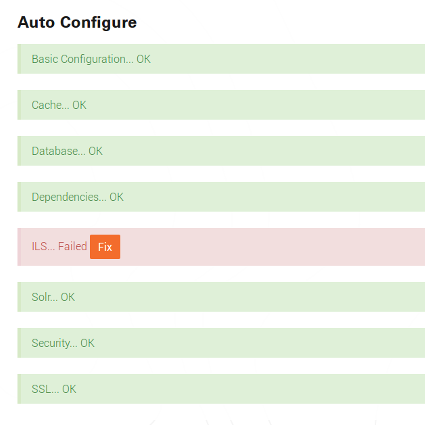
\includegraphics[width=0.6\textwidth]{auto-conf}
\centering
\caption{Uk�zka automatick� konfigurace VuFindu v N�rodn� technick� knihovn�.}
\label{fig:auto-conf}
\end{figure}

V tuto chv�li je VuFind p�ipraven k implementaci konkr�tn�ch pot�eb knihovny a p�izp�soben� dan�mu prost�ed�. \cite{vufind.org}


\section{Implementace}
\label{sec:implementace}
Zde jest pops�no dal�� nastaven� na�eho serveru (nikoli nejnutn�j�� z�kladn� popsan� v p�edchoz� verzi).

Instalace Shibboleth, Cron,..
\subsection{Kustomizace}
\label{sec:kustomizace}
Vzhled u�ivatelsk�ho rozhran� je prvn� v�c, kter� z�kazn�ka prohl�ej�c�ho katalog zaujme. Proto je t�eba kl�st na toto t�ma d�raz. Krom� grafick�ho designu je velmi d�le�it� rozlo�en� jednotliv�ch prvk� na str�nce. Discipl�na, kter� se t�mto zab�v� se naz�v� User Experience. Db� na to, aby se u�ivatel webov� str�nky c�til pohodln� p�i jej�m prohl�en� a z�rove� intuitivn� nach�zel, co pot�ebuje. \cite{ux}

Vizu�ln� vzhled katalogu VuFind NTK koresponduje s grafick�m designem webov�ch str�nek knihovny. Snahou knihovny je m�t jednotn� vzhled cel� sv� webov� prezentace, tak�e i ostatn� knihovn� syst�my dostupn� v s�ti internet, jako je nap��klad N�rodn� �lo�i�t� �ed� literatury, maj� tendenci vypadat graficky stejn�, pokud to jenom jde. Grafick� vzhled webov�ch str�nek NTK vyu��v� souboru vizu�ln�ch n�stroj� s n�zvem Bootstrap. Tento grafick� framework vyu��v� technologie HTML, CSS a JS a pou��v� se k vytv��en� responzivn�ch webov�ch projekt�. \cite{bootstrap}


Port�l VuFind ve slo�ce ko�enov�ho adres��e
\begin{verbatim}
/var/www/vufind/themes
\end{verbatim}
nab�z� hned n�kolik vizu�ln�ch variant, jak m��e ve v�choz�m nastaven� katalog vypadat. Jednotliv� mo�nosti rozd�leny do podadres��� p�edstavuj� dal�� grafick� frameworky:
\begin{itemize}
\item blueprint
\item bootprint
\item bootprint3
\item bootstrap
\item bootstrap3
\item jquerymobile
\end{itemize}


Prvn�m krokem k vytvo�en� vlastn�ho grafick�ho t�matu NTK je zkop�rov�n� cel�ho adres��e \texttt{bootstrap3} do nov�ho adres��e \texttt{ntk}. V tomto nov�m adres��i je t�eba editovat a upravit dle pot�eby soubor \texttt{theme.config.php}, kter� nese informace o tom, jak� pomocn� skripty a soubory se na��taj� pro spr�vn� vykreslen� webov�ch str�nek. Vzhledem k tomu, �e pro prost�ed� NTK byly vytvo�eny vlastn� CSS soubory, jsou to pr�v� ony, k nim� se zde zapisuje cesta. Dal��mi soubory pro z�pis jsou javascripty. N�kter� p�vodn� jsou upraveny, jin� jsou zcela nov� p�id�ny kv�li lok�ln�m pot�eb�m. P��kladem p�idan�ho javascriptu je \texttt{NTK.js}, kter� obsluhuje komunikaci se slu�bou Obalkyknih.cz. Tato slu�ba poskytuje datab�zi naskenovan�ch ob�lek a obsah� knih, kterou vyu��vaj� i do kter� p�isp�vaj� knihovny a kni�n� nakladatelstv� po cel� �esk� republice.

V podadres��i \texttt{templates} jsou dle v�znamu jednotliv�ch sekc� ulo�eny ve slo�k�ch �ablony, kter� definuj� jak bude dan� webov� str�nka vypadat. Tyto �ablony jsou ve form�tu \texttt{phtml}, kter� do nich umo��uje zapisovat obsah jednak v jazyce HTML, tak tak� v jazyce PHP. Soubor \texttt{header.phtml} definuje vzhled z�hlav� str�nek a soubor \texttt{footer.phtml} naopak definuje, jak bude vypadat z�pat� str�nek. Hlavn� rozvr�en� str�nek je definov�no v souboru \texttt{layout/layout.phtml}. Dal�� slo�kou, kter� proch�z� zna�nou �pravou je \texttt{record}, kter� obsahuje �ablony nastavuj�c� vzhled zobrazen� detailn�ho n�hledu z�znamu v katalogu, v�etn� �ablon pro odesl�n� z�znamu e-mailem, ulo�en� ho do u�ivatelsk�ho konta, citov�n� z�znamu, atd. Pro citov�n� z�znam� je zde napojena slu�ba CitacePro.com, d�ky jej�mu� api rozhran� lze zobrazovat citace z�znam� p��mo v katalogu Vufind. Zaj�mav� slo�ka se �ablonami, kter� tak� souvis� s detailn�m n�hledem z�znamu, je \texttt{RecordTab}. V n� se definuj� z�lo�ky, kter� se u z�znamu zobraz�. Krom� b�n�ch z�lo�ek Jednotky, Popis, Koment��e, MARC je pro prost�ed� NTK p�id�na z�lo�ka pops�na v �ablon� \texttt{preview.phtml}. Ta se zobrazuje pouze u z�znam� obohacen�ch o naskenovan� n�kter� ��sti d�la. V z�lo�ce je tedy k dispozici n�hled t�chto sken� ulo�en�ch na serveru Aleph, kter� u�ivateli p�edstavuje uk�zku p�ibli�uj�c� obsah dan�ho exempl��e. Zdrojov� k�d t�to �ablony je:
\begin{lstlisting}
<?
// Set page title.
$this->headTitle($this->translate('Preview') . ': ' . $this->driver->getBreadcrumb());
$id = $this->driver->getUniqueID();
// Links with pictures on this site
$addr = 'http://aleph.techlib.cz/cgi-bin/obrazek.pl?sn='.$id;
$links = file_get_contents( $addr );
// Pattern starts with "http" and ends with ".jpg" or ".JPG"
$pattern = '/http.{0,100}\.(JPG|jpg)/';
// Each link in 2D-array named url
$count = preg_match_all( $pattern, $links, $url);
// One array for small and one for big pics
$pics= array();
$thumbs= array();
for ($i=0; $i<$count; $i++){
        // is this thumbnail ?
        if (strpos($url[0][$i], 'thumb')){
                $thumbs[$i]=$url[0][$i];
        }else{
                $pics[$i]=$url[0][$i];
        }
}
// Alphabetical sorting
sort($pics);
sort($thumbs);
?>
<? foreach ($thumbs as $key => $value): ?>
    <a href=<?=$pics[$key]?>><img src=<?=$thumbs[$key]?>></a>
<? endforeach; ?>
\end{lstlisting}
Pro rozvr�en� v�sledk� vyhled�v�n� slou�� �ablona:
\begin{lstlisting}
RecordDriver/SolrDefault/result-list.phtml
\end{lstlisting}
Ve stejn�m um�st�n� se nach�z� �ablona \texttt{core.phtml}, kter� se zobrazuje v detailu z�znamu a na��t� informace o dan�m z�znamu z MARCov�ch pol�, pop��pad� z indexu nebo z lok�ln� datab�ze katalogu. T�mito �daji jsou autor, form�t, jazyk, vydavatelstv�, edice, t�mata, on-line p��stup a u�ivatelsk� tagy. Za zm�nku jist� stoj� slo�ka \texttt{search}, kter� obsahuje �ablony t�kaj�c� se vyhled�v�n� v �ir��m slova smyslu. Jsou to nap��klad �ablona na zobrazen� historie vyhled�van� \texttt{history.phtml}, d�le �ablona \texttt{email.phtml} zobrazuj�c� formul�� pro odesl�n� vyhled�v�n� e-mailem, �ablona na zobrazen� vyhled�vac�ho pole \texttt{searchbox.phtml} a tak� jsou zde �ablony pokro�il�ho vyhled�v�n�. Slo�ka \texttt{myresearch} obsahuje �ablony t�kaj�c� se u�ivatelsk�ho konta, kter� jsou samoz�ejm� tak� upraveny tak, aby zapadaly do jednotn�ho grafick�ho konceptu. Nej�ast�j��mi �pravami ve�ker�ch zobrazuj�c�ch se �ablon je zm�na rozvr�en� str�nky ve smyslu �pravy velikosti ���ek a v��ek jednotliv�ch sloupc�, ��dk�, zarovn�n�, tla��tek, nadpis�, tabulek, seznam�, ohrani�en�, atd. pomoc� soubor� s kask�dov�mi styly. \cite{ui}


\subsection{WorkFlow}
\label{sec:workflow}
Redmine - issue tracker. Zad�v�n� �kol�. �e�en�. Repozit��. Nejprve se zm�ny provedou na testovac� verzi. N�kolik dn� se testuje. Potom p�enos na produk�n� verzi.
\section{Provoz}
\label{sec:provoz}
Popis b�n�ho provozu. Statistiky n�v�t�vnosti. Vyhled�vac� v�razy. Ka�dodenn� harvestov�n� - Cron. Google Analytics.

podkapitoly Statistiky a Workflow

popis mechanismu cronu - sklizen� import start...


robots.txt, sitemap

\chapter{Dal�� Open source software}
\label{sec:chapter02}
Filozofie open source. 
Open source software 

Pojmem open source lze ozna�it cokoli, co je mo�n� upravit a d�le sd�let d�ky ve�ejn� p��stupnosti. I kdy� toto ozna�en� vzniklo v souvislosti s rozvojem po��ta�ov�ho software, dnes se term�n pou��v� tak� pro projekty, produkty, iniciativy, kter� ct� hodnoty jak�mi jsou otev�en� v�m�na, kooperativn� spolupr�ce, transparentnost, meritokracie, rapid prototyping a komunitn� rozvoj.

Open source software, je takov� software, jeho� zdrojov� k�d je dostupn� komukoliv za ��elem jeho zlep�en� �i jak�koliv jeho modifikace.

Zdrojov� k�d je ��st software, kterou v�t�ina u�ivatel� po��ta�e v�bec nevid�; je to k�d, kter�m po��ta�ov� program�to�i mohou manipulovat tak, aby m�nili chov�n� dan�ho programu �i aplikace. Program�to�i, kte�� maj� p��stup k zdrojov�mu k�du po��ta�ov�ho programu jej mohou vylep�ovat p�id�n�m funkcionality nebo opraven�m ��st�, kter� ne v�dy funguj� spr�vn�.
https://opensource.com/resources/what-open-source

Open source software,  v �esk�m p�ekladu software s otev�en�m zdrojov�m k�dem, n�kdy ozna�ov�n i jako svobodn� software v�ak nutn� neznamen�, �e jeho u�it� je zcela zdarma. Proto ned�lnou sou��st� tohoto typu softwaru je licencov�n�, kter� stanovuje podm�nky nakl�d�n� s dan�m programem.
http://www.gnu.org/philosophy/free-software-for-freedom.cs.html

Existuje mnoho rozd�ln�ch typ� licenc� pro svobodn� software. N�kter� softwary pou��vaj� autorsk� pr�vo zp�sobem copyleft. To umo��uje ���en� svobodn�ho software ve ve�ejn�m prostoru bez rizika, �e se po jeho jak�koli ��ste�n� modifikaci stane softwarem propriet�rn�m, tedy uzav�e se jeho zdrojov� k�d a jeho pou�it� se zpoplatn�n�. https://www.gnu.org/copyleft/
P�edn�m z�stupcem takov�ho typu licenc� je licence GNU GPL (GNU General Public License), kter� tedy chr�n� svobodu svobodn�ho po��ta�ov�ho programu i po jeho modifikaci a ukl�d� tak u�ivatel�m povinnost ���it odvozen� d�lo pod stejnou licenc�.
\url{http://www.webopedia.com/DidYouKnow/Computer_Science/open_source.asp}
Celou oblast svobodn�ho software zast�e�uje neziskov� korporace Open Source Initiative (OSI) zalo�en� v roce 1998 se s�dlem v Kalifornii, kter� vytv��� licence, definuje open source a p��slu�n� standardy.
https://opensource.org/
V�voj konkr�tn�ho open source software obvykle vede jedna konkr�tn� spole�nost, kter� se rozhodne pro zp�sob v duchu spolupr�ce a distribuovan� �innosti. T�m se projekt rozjede, t�eba i za finan�n� podpory.\cite{vufind.oblibene}
Postupem �asu, d�ky ve�ejn�mu ���en�, se za��n� vytv��et komunita participuj�c�ch v�voj���, kte�� na�li ve vznikaj�c�m produktu smysl a pr�ce se tak m��e st�t dobrovolnou, tedy radostnou a plodnou. V p��pad� d�l��ch �sp�ch� p�ib�vaj�c� potenci�l st�le roste. Nejinak tomu bylo i v open source projetu VuFind. Ten vznikl na akademick� p�d� v USA a dnes m� �irokou komunitu p�isp�vatel� po cel�m sv�t�, kter� ��t�
okolo 70 aktivn�ch �len�. 
https://github.com/vufind-org/vufind/graphs/contributors

mailing-list



potom Evergreen, 
Evergreen je knihovn� software
\cite{evergreen.ctenar}

Koha
hostingov� server pro open source projekty
https://sourceforge.net
Docela dobr� p�edstaven� nejen VuFindu.
http://ikaros.cz/opacy-nove-generace-ii-%E2%80%93-virgobeta-a-vufind

\chapter{Pou�it� VuFindu v ostatn�ch knihovn�ch (�R, zahrani��)}
\label{sec:chapter04}

VuFind je nasazen v relativn� hodn� instituc�ch po cel�m sv�t�, a� u� jako produk�n� server (cca 120 instalac�) nebo jako server testovac� (cca 20 instalac�). D�ky tomu je mo�n� vid�t, jak lze tento syst�m pou��vat mnoha r�zn�mi zp�soby a upravovat. N�kter� p��klady jsou uvedeny d�le. \cite{vufind.org.installations}

Bibliographies at arthistoricum.net je n�meckou akademickou instituc� provozuj�c� VuFind 3.0.1 na linuxov� distribuci opera�n�ho syst�mu Ubuntu. Jej� vizu�ln� prezentace vych�z� z t�matu Bootstrap3.

\begin{figure}[h]
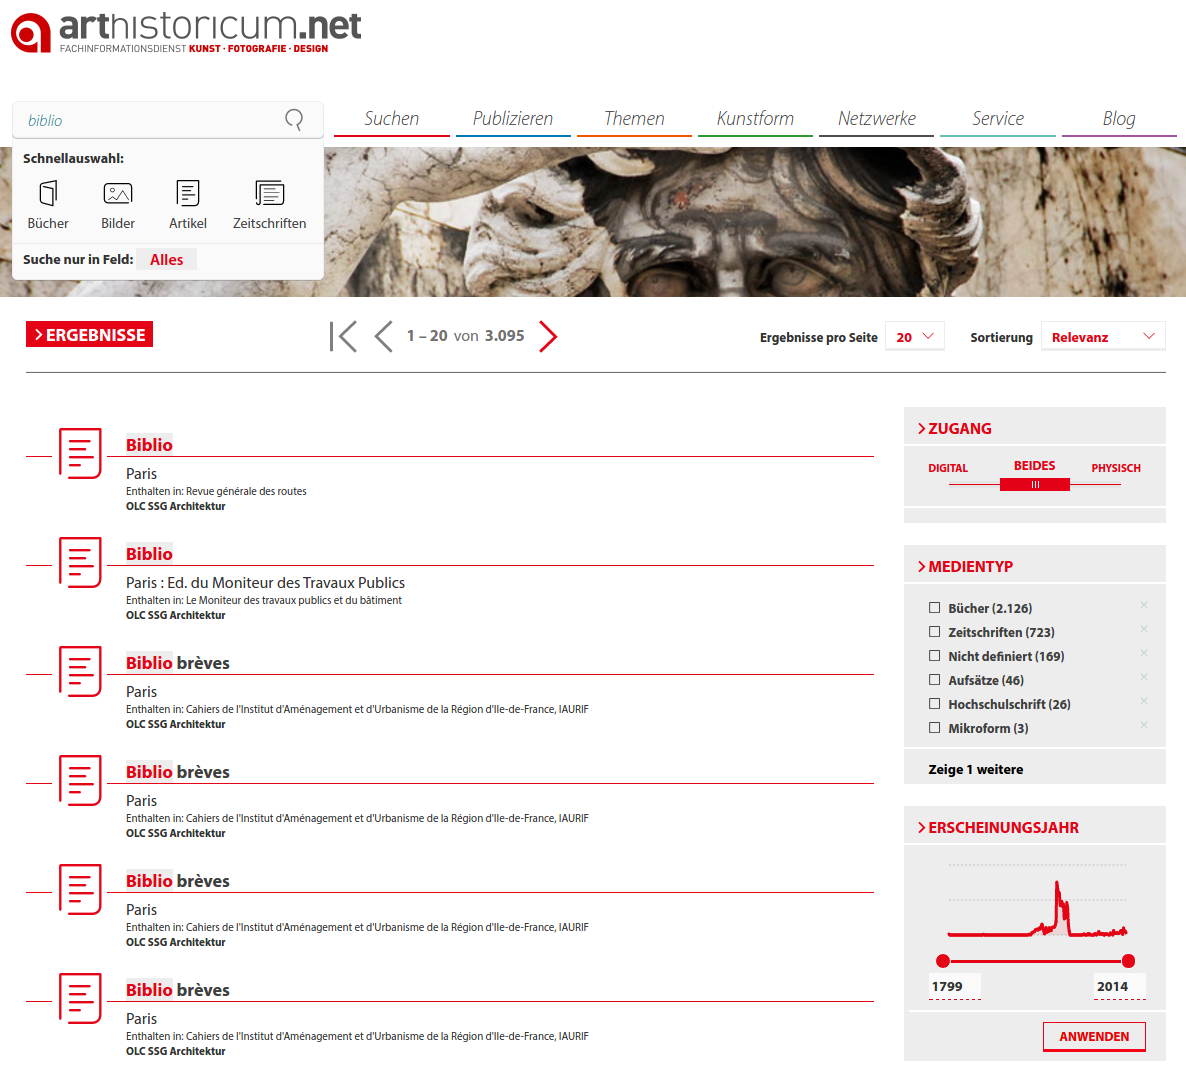
\includegraphics[width=0.7\textwidth]{vufind-1}
\centering
\caption{Uk�zka on-line katalogu n�meck� knihovny Bibliographies at arthistoricum.net dostupn�ho na \url{http://www.arthistoricum.net/subjects/bibliographies/}.}
\label{fig:vuf1}
\end{figure}

Dal�� akademickou instituc� pou��vaj�c� VuFind v nejnov�j�� stabiln� verzi 3.0.1 je pochopiteln� Villanova University, v jej� knihovn� VuFind vznikl. Tato americk� univerzita pou��v� jako opera�n� syst�m pro provoz VuFindu linuxovou distribuci RedHat. V prost�ed� t�to knihovny je VuFind rozhran�m pro integrovan� knihovnick� syst�m Voyager a z�rove� pro discovery syst�m Summon. Vizualn� vzhled op�t vych�z� ze standardizovan�ho t�matu Bootstrap3.

\begin{figure}[h]
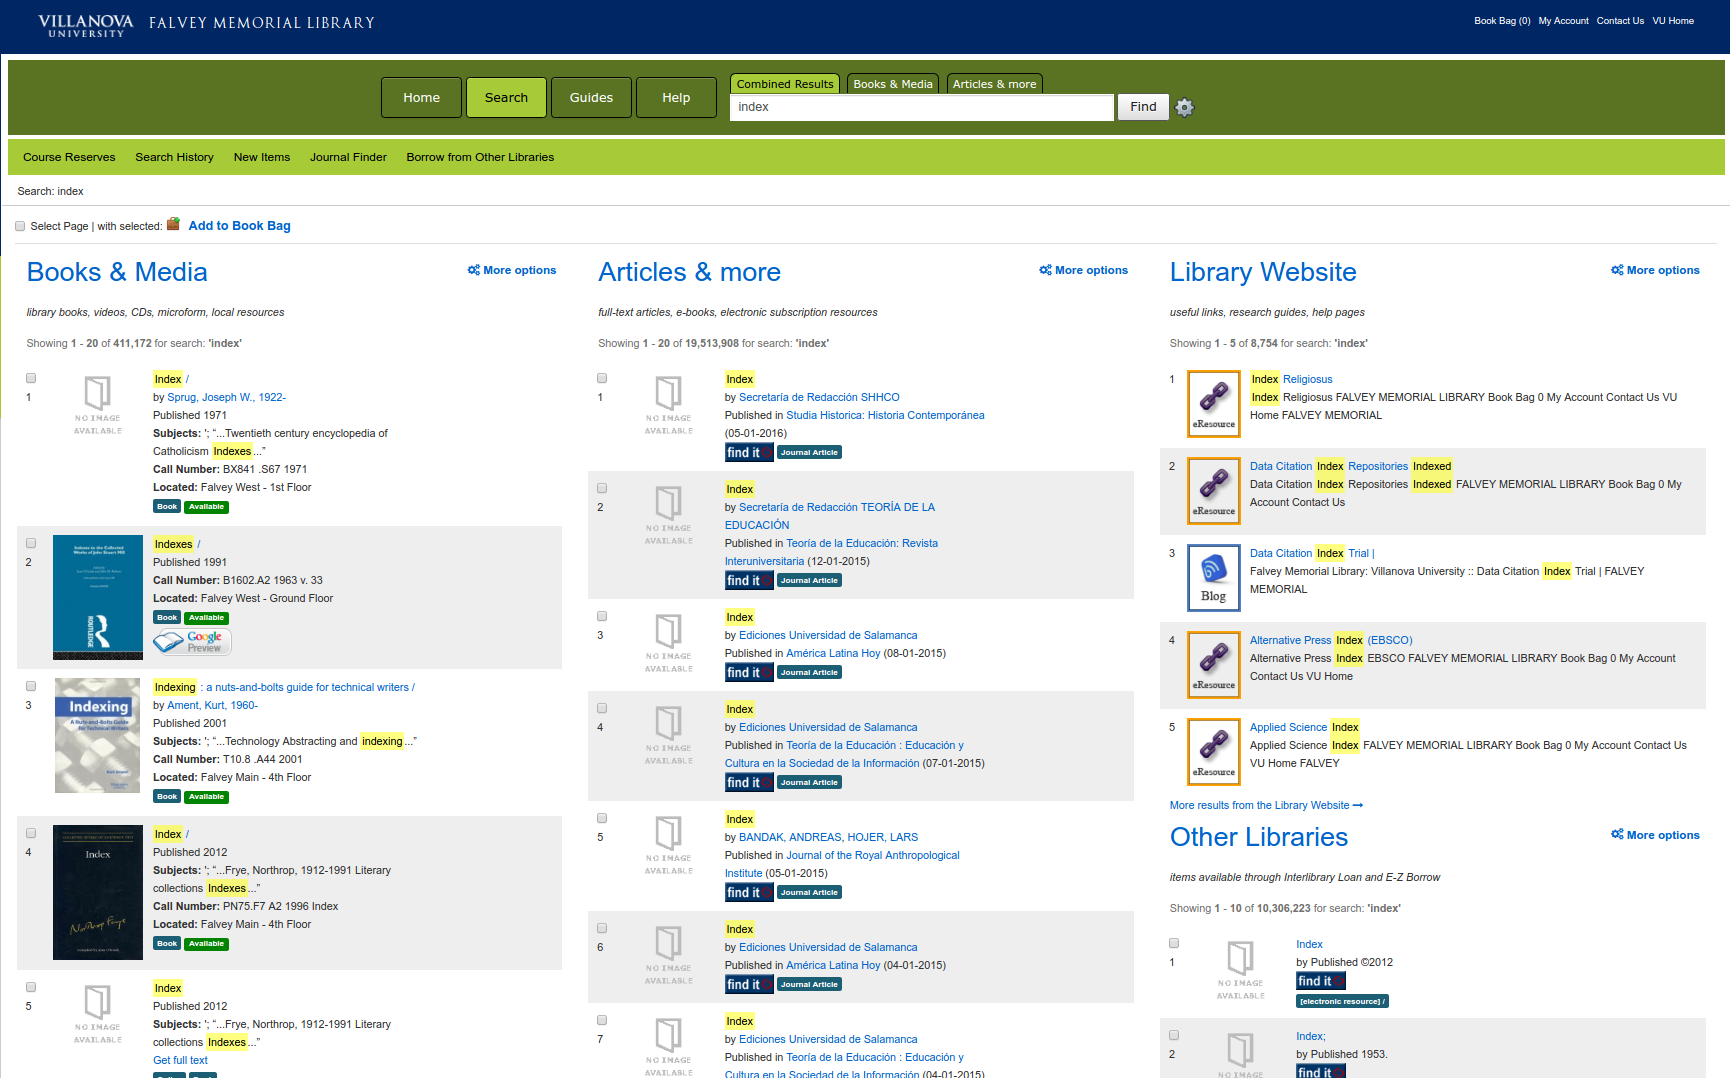
\includegraphics[width=0.7\textwidth]{vufind-2}
\centering
\caption{Uk�zka on-line katalogu americk� knihovny Villanova University dostupn�ho na \url{https://library.villanova.edu/Find/}.}
\label{fig:vuf2}
\end{figure}

Rusk� univerzita Perm National Research Polytechnic University tak� pou��v� pro vyhled�v�n� a proch�zen� sv�ch zdroj� t�m�� nejnov�j�� verzi, tedy VuFind 3.0. Opera�n�m syst�mem je v tomto p��pad� Windows a napojen� na integrovan� knihovnick� syst�m Ruslan spole�n� s napojen�m na discovery syst�m EBSCO Discovery je zahaleno v h�vu t�matu Bootstrap3. Tato instalace ov�em na rozd�l od p�edchoz�ch p��pad� nen� pravd�podobn� nasazen� v produk�n�m re�imu, n�br� v m�du testovac�m. Nicm�n� i tak je dostupn� p�es s� internet.

\begin{figure}[!htb]
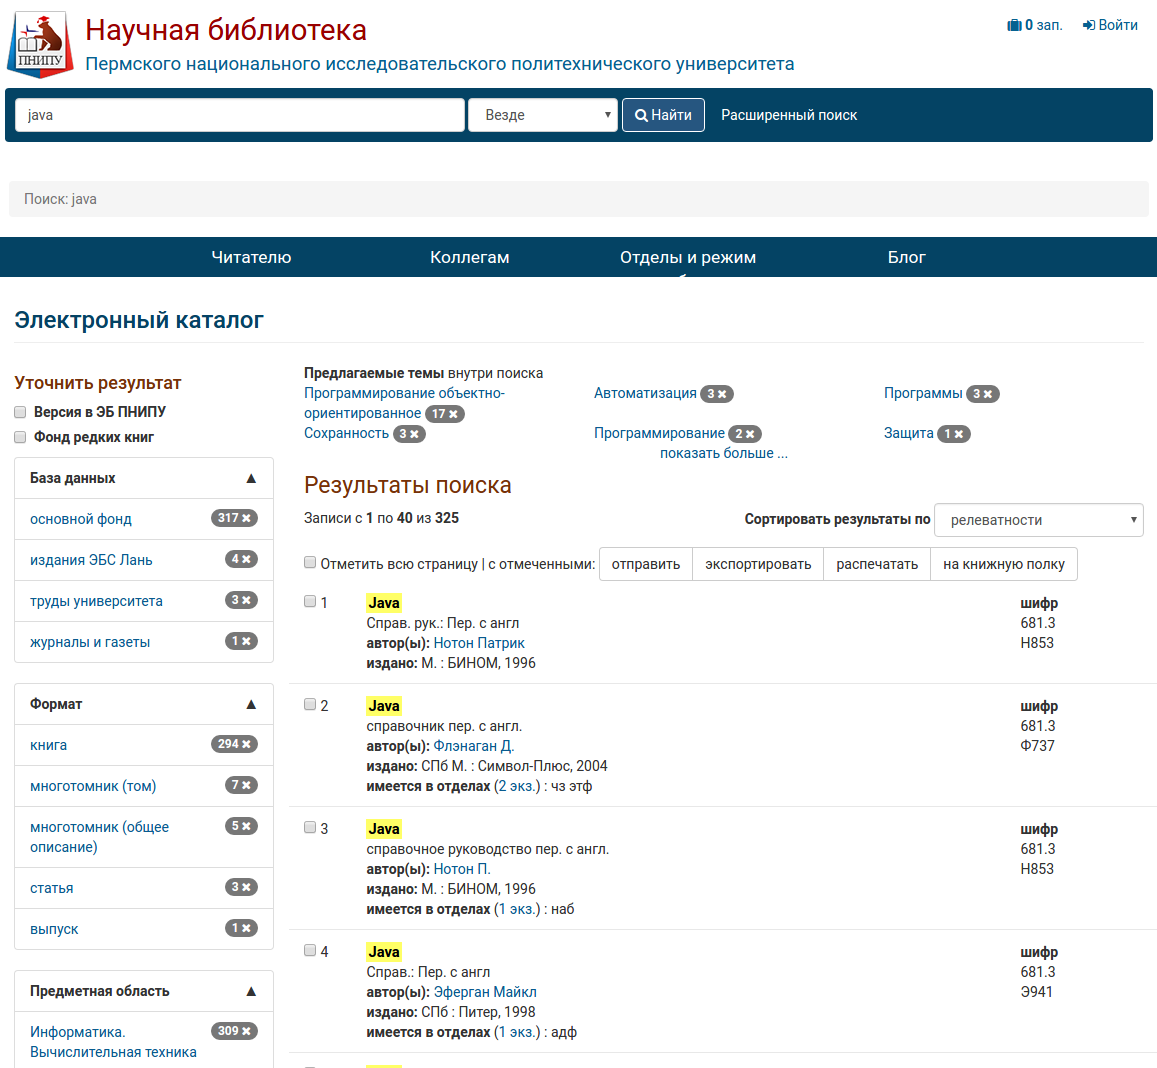
\includegraphics[width=0.7\textwidth]{vufind-3}
\centering
\caption{Uk�zka on-line katalogu rusk� univerzitn� knihovny Perm National Research Polytechnic University dostupn�ho na \url{http://elib.pstu.ru/vufind/}.}
\label{fig:vuf3}
\end{figure}

\begin{figure}[!htb]
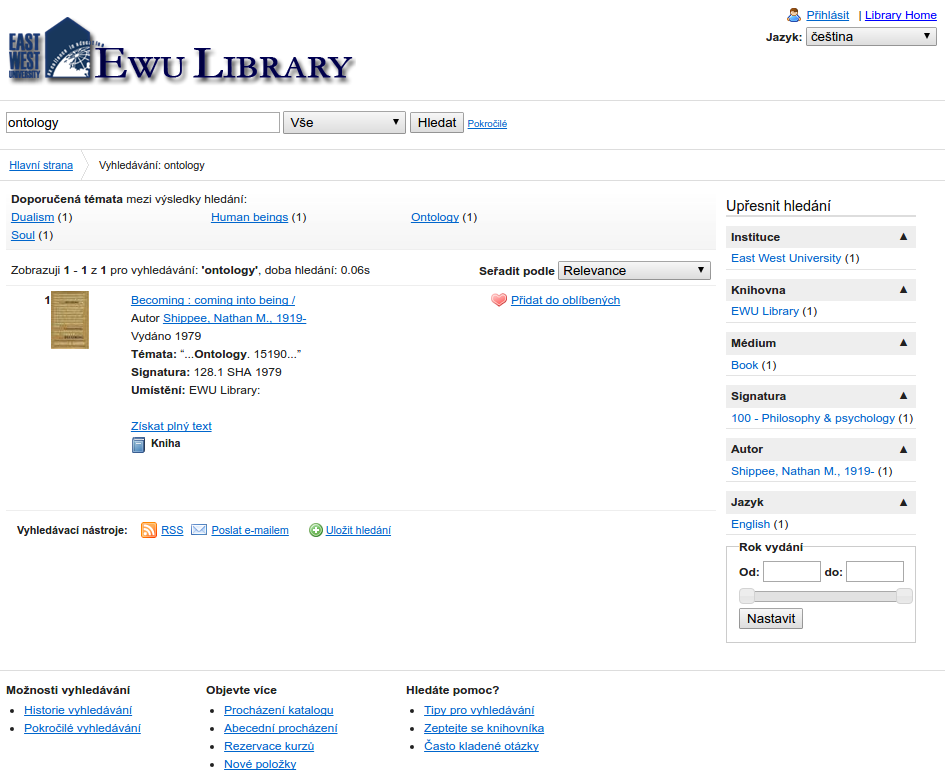
\includegraphics[width=0.7\textwidth]{vufind-4}
\centering
\caption{Uk�zka on-line katalogu univerzitn� knihovny East West University Library v Banglad�i dostupn�ho na \url{http://lib.ewubd.edu/vufind/}.}
\label{fig:vuf4}
\end{figure}

V Dh�ce, hlavn�m m�st� Banglad�e, pou��vaj� VuFind 2.2.1 v knihovn� East West University Library. B�� na linuxov� distribuci opera�n�ho syst�mu Debian a jako integrovan� knihovnick� syst�m pou��v� svobodn� software Koha.

Zaj�mavou instituc� je tak� italsk� univerzita se s�dlem v ��m� Roma Tre University. Instalaci jej�ho port�lu VuFind provedla a d�le spravuje firma Cineca, kter� je v�znamnou firmou s dlouholetou tradic� zab�vaj�c� se informa�n�mi technologiemi v It�lii. Opera�n� syst�m Linux s integrovan�m knihovnick�m syst�mem Aleph a discovery syst�mem Summon v kombinaci s verz� VuFindu 2.3.1 a v�choz�m grafick�m t�matem Bootstrap3 vytv��� velmi podobn� prost�ed� jak� je v N�rodn� technick� knihovn�. 

\begin{figure}[h]
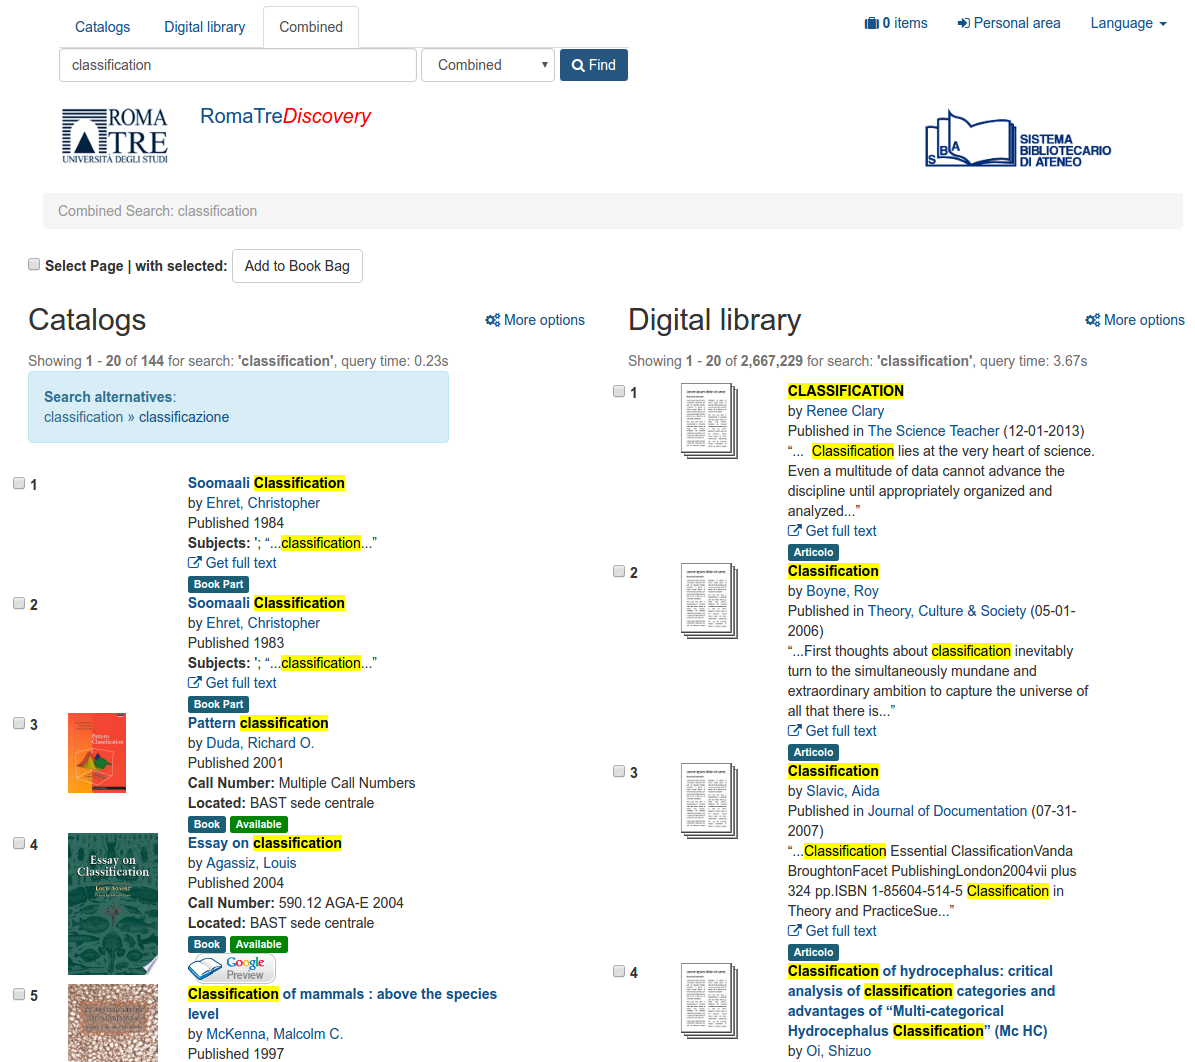
\includegraphics[width=0.7\textwidth]{vufind-5}
\centering
\caption{Uk�zka on-line katalogu univerzitn� knihovny Roma Tre University dostupn�ho na \url{https://discovery.sba.uniroma3.it/}.}
\label{fig:vuf5}
\end{figure}

Dal�� zaj�mavou instalaci port�lu VuFind m� s� �v�carsk�ch univerzitn�ch knihoven kolem m�st Basilej a Bern zvan� Swissbib Basel Bern. Stejn� jako v N�rodn� technick� knihovn� i zde b�� vyhled�v�n� na linuxov� distribuci opera�n�ho syst�mu RedHat spole�n� s integrovan�m knihovnick�m syst�mem Aleph a discovery syst�mem Summon. Vzhed je rovn� odvozen od t�matu Bootstrap3. P�ed n�kolika dny zde byla implementov�na nejnov�j�� verze Vufindu 3.0.1. Zdrojov� k�d je dostupn� p�es webovou slu�bu GitHub na \url{https://github.com/swissbib/vufind}.

\begin{figure}[!htb]
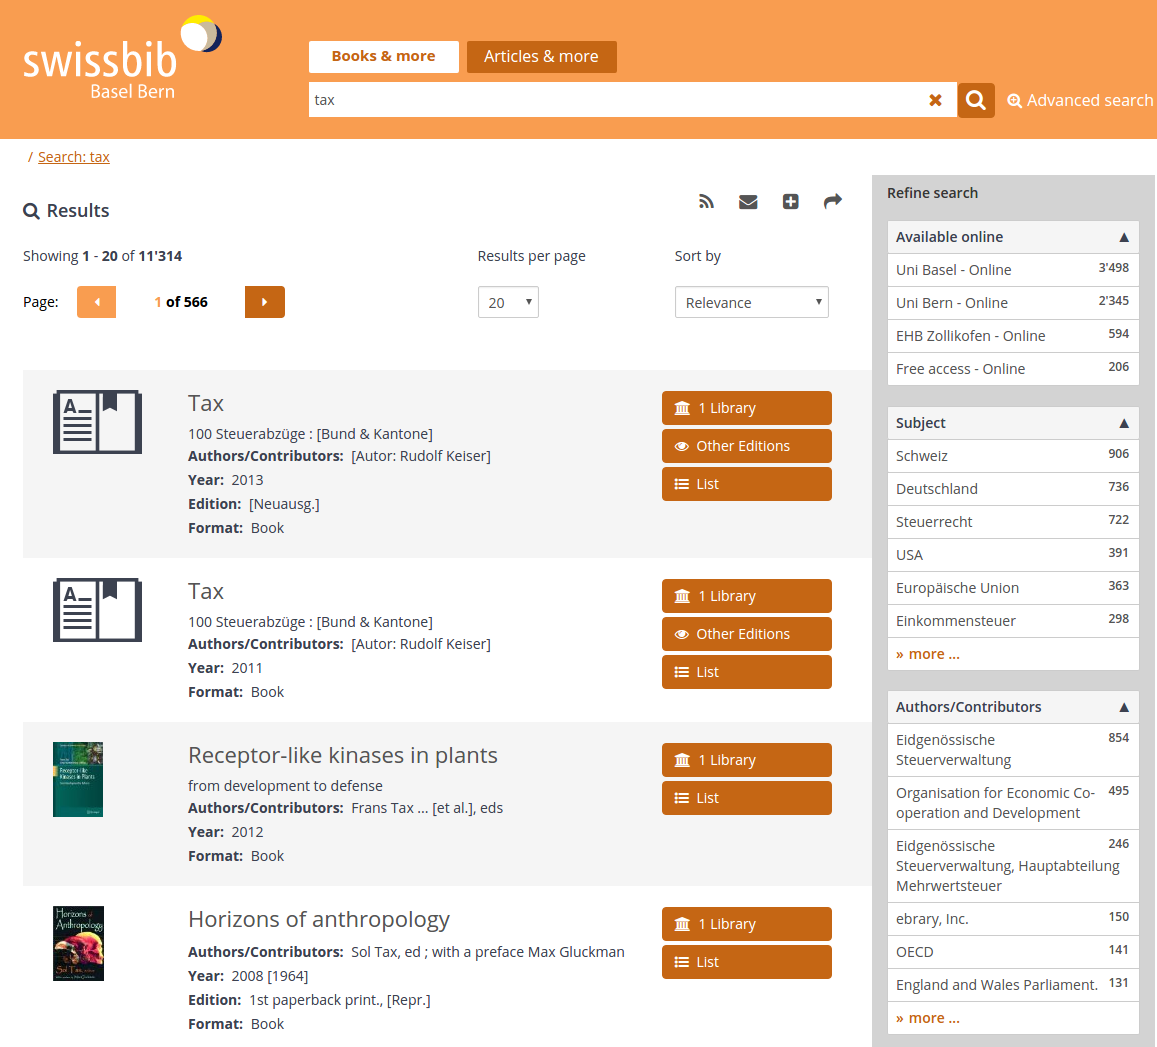
\includegraphics[width=0.67\textwidth]{vufind-6a}
\centering
\caption{Uk�zka on-line katalogu Swissbib Basel Bern p�i vyhled�v�n� v lok�ln�m fondu knihovny dostupn�ho na \url{http://baselbern.swissbib.ch/}.}
\label{fig:vuf6a}
\end{figure}

\begin{figure}[!htb]
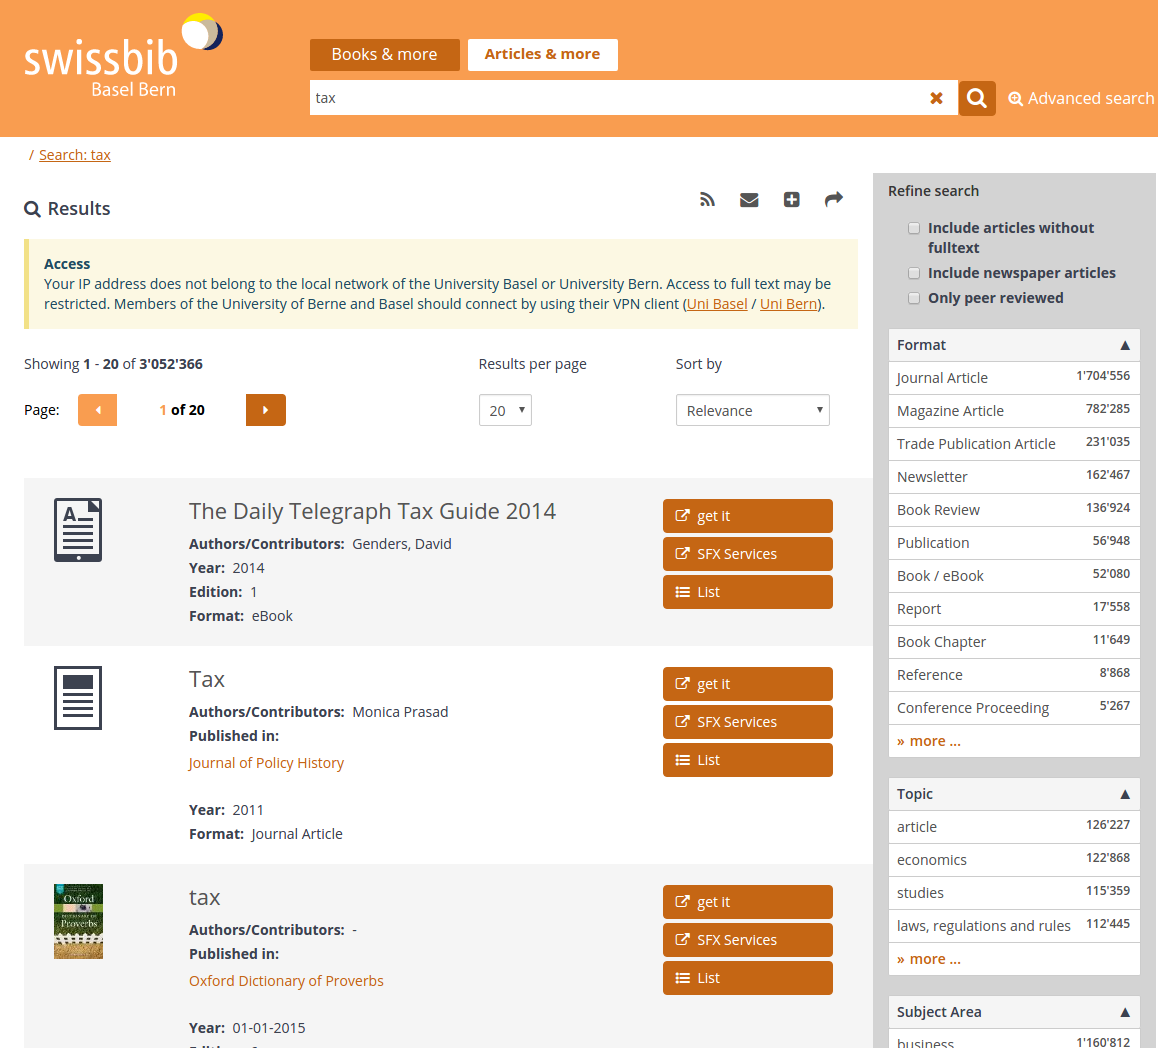
\includegraphics[width=0.67\textwidth]{vufind-6b}
\centering
\caption{Uk�zka on-line katalogu Swissbib Basel Bern p�i vyhled�v�n� v elektronick�ch zdroj�ch knihovny dostupn�ho na\url{http://baselbern.swissbib.ch/}.}
\label{fig:vuf6b}
\end{figure}

Za pozornost stoj� i tureck� univerzitn� knihovna Suleyman Demirel University Library s VuFindem 2.3.1. Opera�n�m syst�mem je zde linuxov� distribuce CentOS, discovery syst�mem je Summon a integrovan�m knihovnick�m syst�mem je svobodn� software Koha. Takov�to kombinace m��e b�t pro N�rodn� technickou knihovnu inspirac�.

\begin{figure}[!htb]
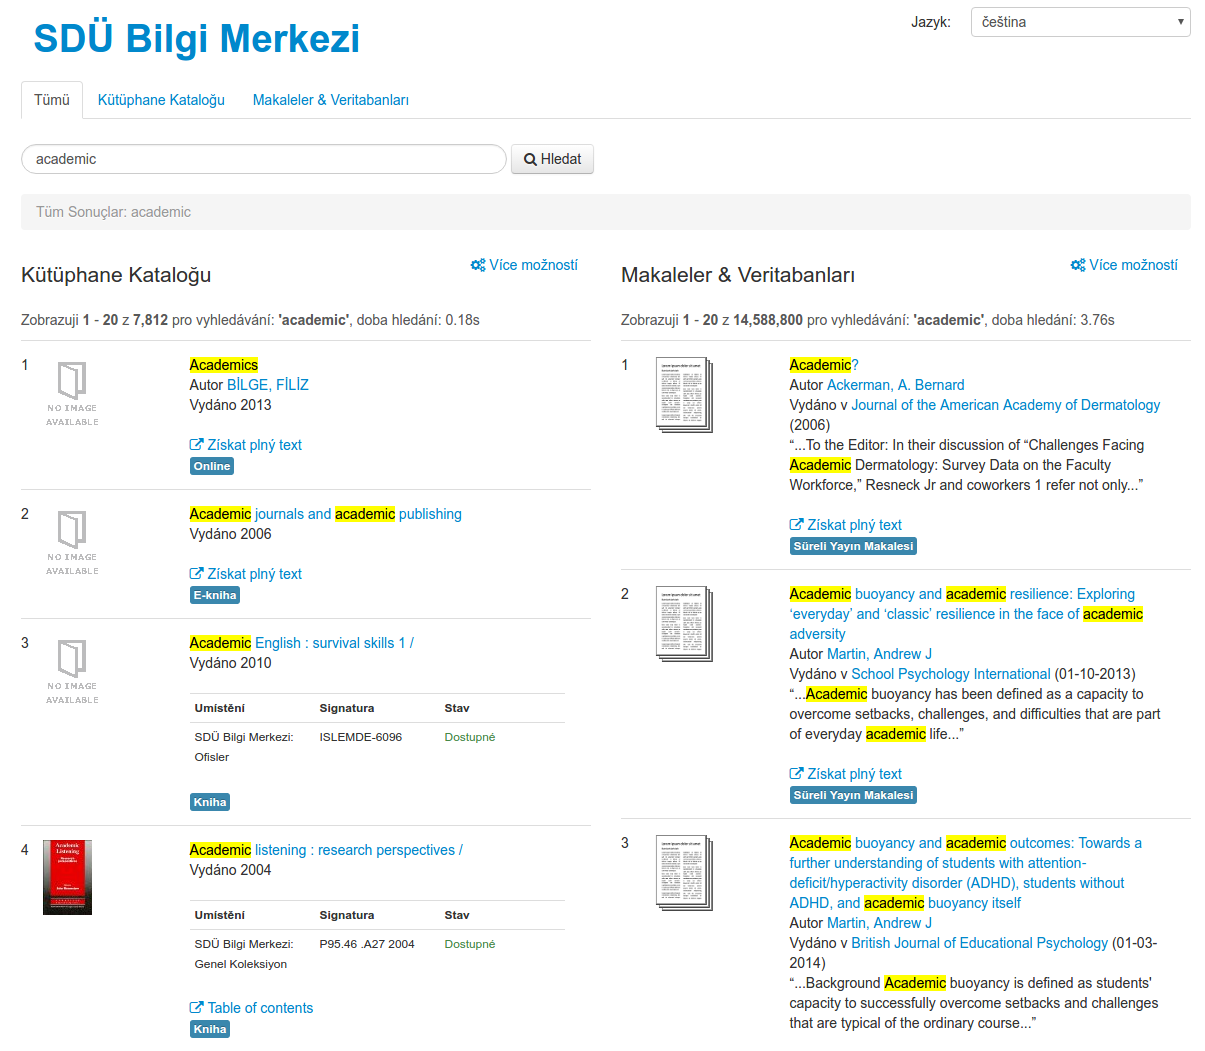
\includegraphics[width=0.7\textwidth]{vufind-7}
\centering
\caption{Uk�zka on-line katalogu univerzitn� knihovny Suleyman Demirel University Library dostupn�ho na \url{http://tara.sdu.edu.tr/vufind/}.}
\label{fig:vuf7}
\end{figure}


Discovery syst�m Primo od firmy ExLibris je do VuFindu napojen ve spole�n�m katalogu pro st�tn� a univerzitn� knihovny v Hamburgu zvan�m Beluga. Toto pojmenov�n� nese analogii s kytovcem B�luhou severn�, kter� m� �dajn� soci�ln� a p��telsk� chov�n� a d�ky tomu je pr�ce s t�mto katalogem u�ite�n� a radostn�. Opera�n�m syst�mem tohoto vyhled�va�e je linuxov� distribuce Suse a integrovan�m knihovnick�m syst�mem OCLC.

\begin{figure}[!htb]
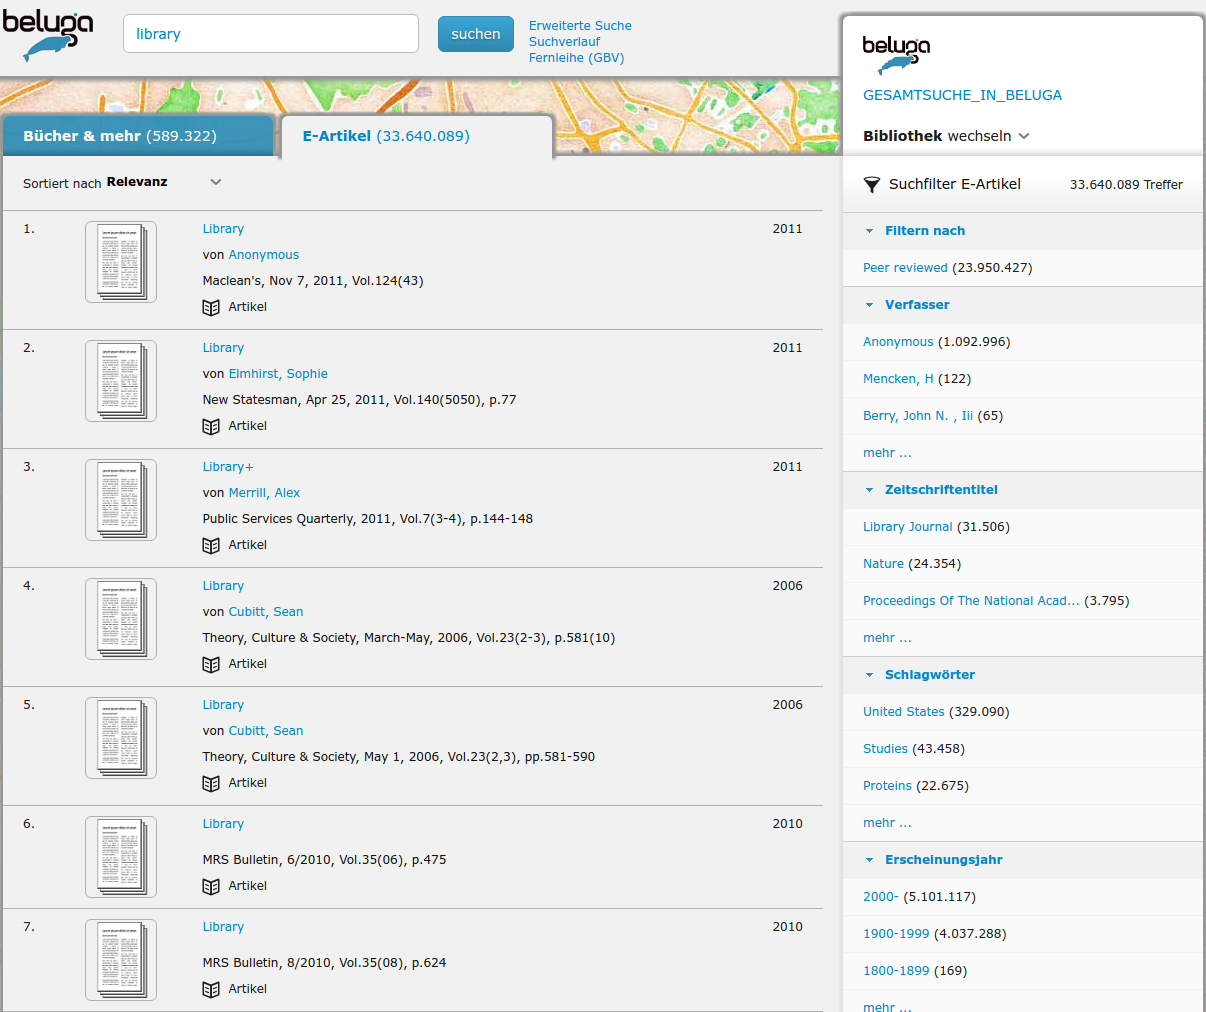
\includegraphics[width=0.7\textwidth]{vufind-8}
\centering
\caption{Uk�zka on-line katalogu Beluga dostupn�ho na \url{https://beluga.sub.uni-hamburg.de/vufind/}.}
\label{fig:vuf8}
\end{figure}

Napojen� discovery syst�mu EBSCO je mo�n� vid�t v katalogu �pan�lsk� univerzitn� knihovny Biblioteca de la Universidad de Oviedo, je� b�� v linuxov� distribuci opera�n�ho syst�mu CentOS s napojen�m na integrovan� knihovnick� syst�m Amicus. 

\begin{figure}[h]
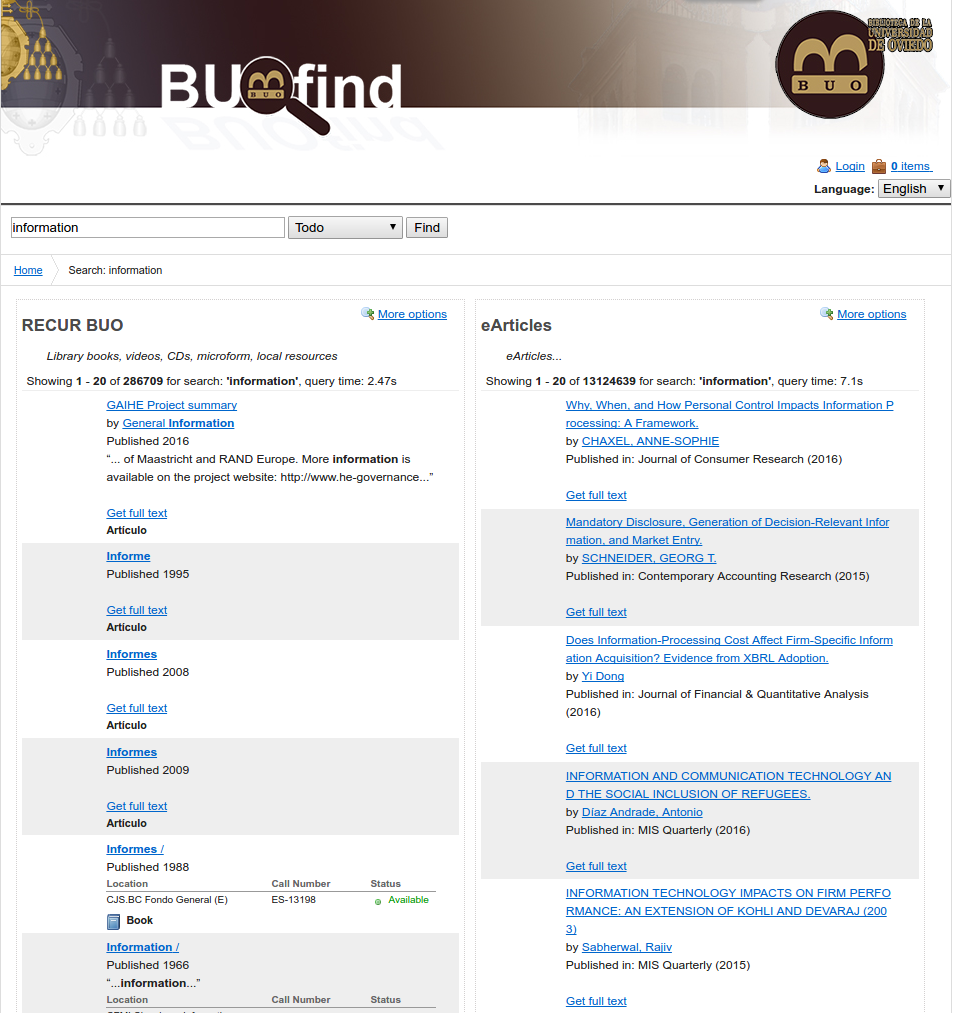
\includegraphics[width=0.7\textwidth]{vufind-9}
\centering
\caption{Uk�zka on-line katalogu �pan�lsk� univerzitn� knihovny Biblioteca de la Universidad de Oviedo dostupn�ho na \url{http://vufind.uniovi.es/}.}
\label{fig:vuf9}
\end{figure}

\begin{figure}[!htb]
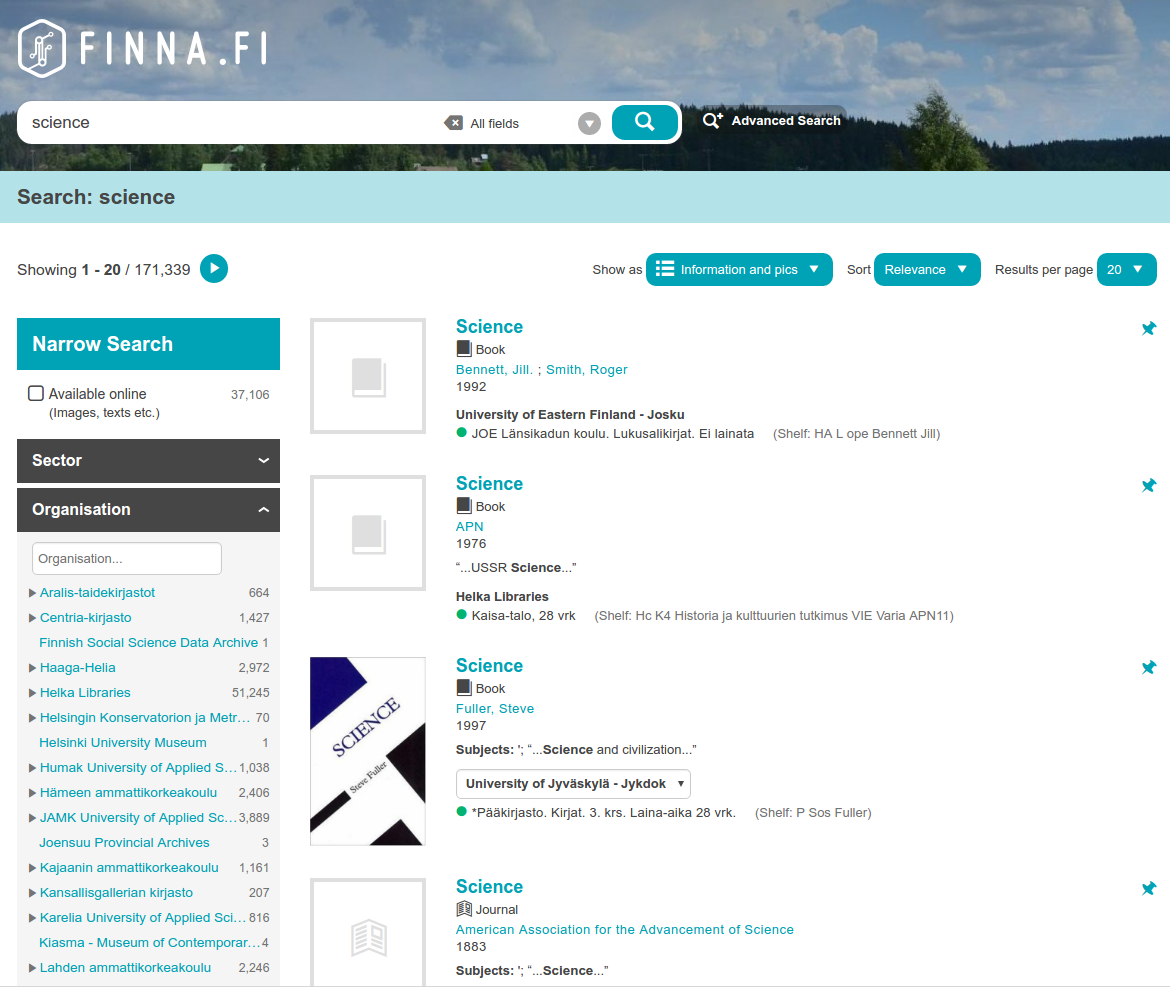
\includegraphics[width=0.7\textwidth]{finna}
\centering
\caption{Uk�zka vyhled�vac�ho rozhran� Finna dostupn�ho na \url{https://finna.fi/}.}
\label{fig:finna}
\end{figure}

\begin{figure}[!htb]
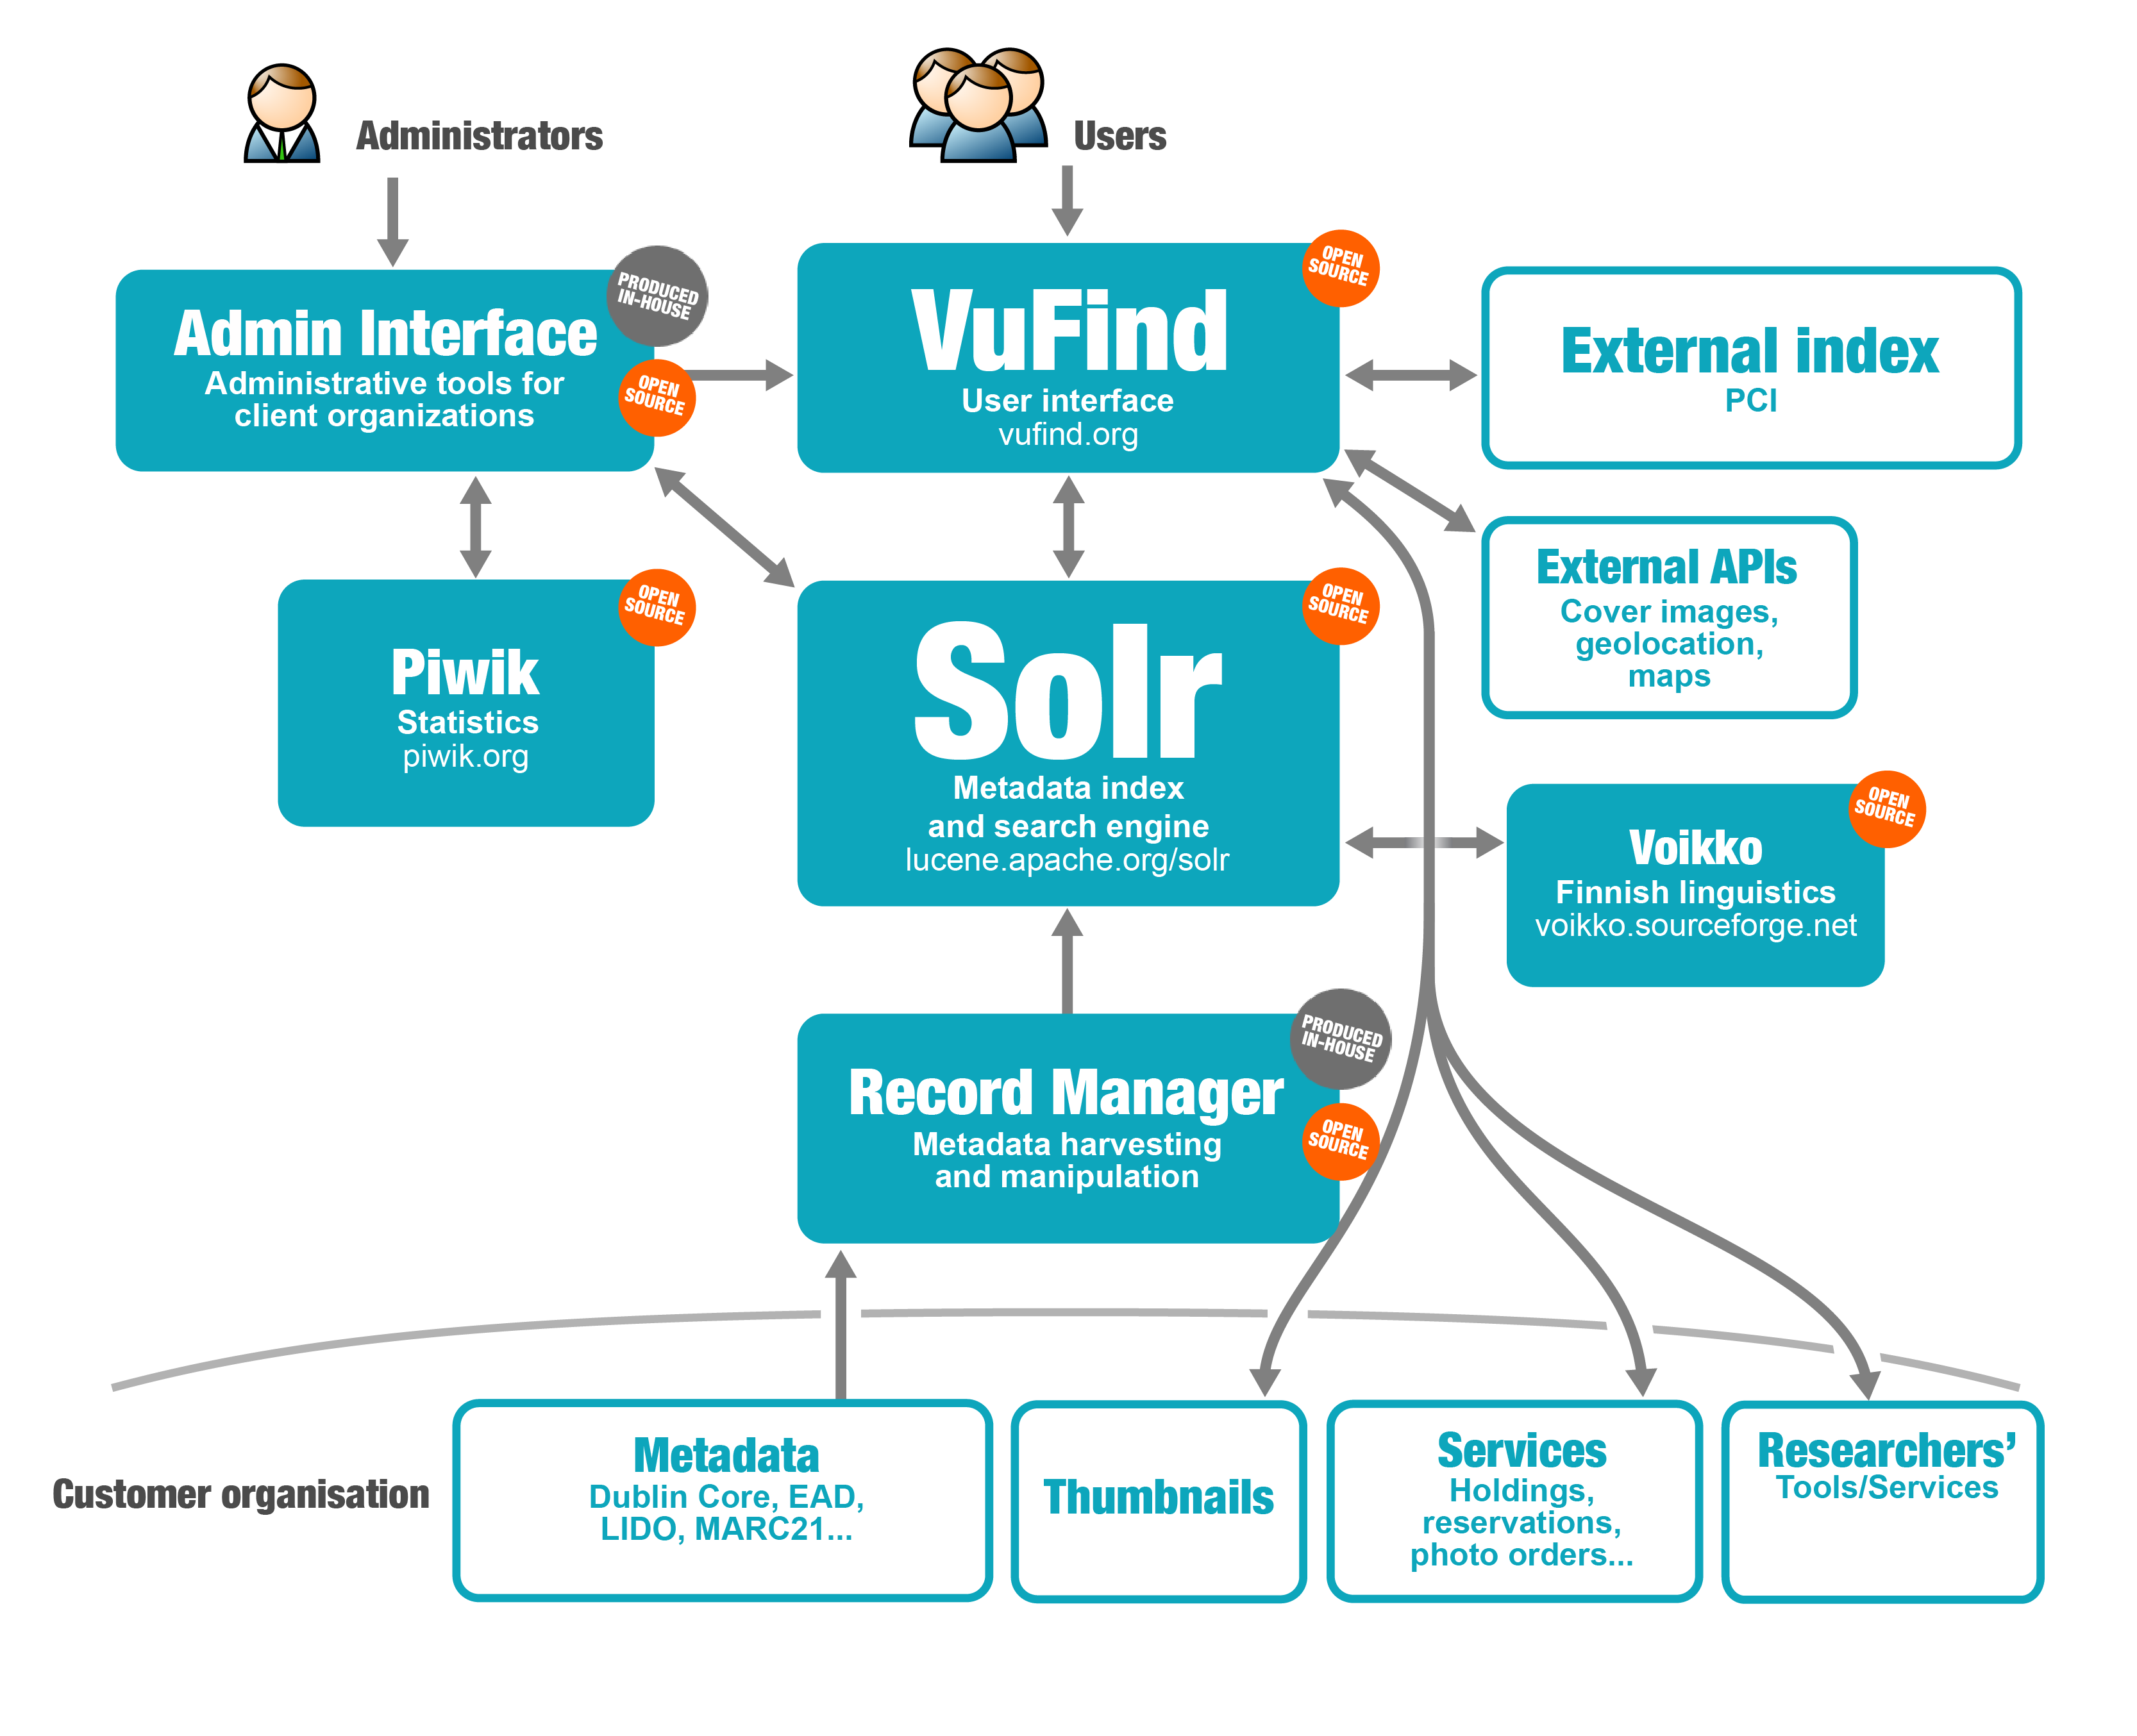
\includegraphics[width=0.7\textwidth]{finna_architecture}
\centering
\caption{Grafick� zn�zorn�n� architektury cel�ho syst�mu Finna ukazuje propojen� jednotliv�ch modul�, p�i�em� jedn�m z nich je VuFind \cite{ndl.vufind}.}
\label{fig:finna-architecture}
\end{figure}

V�razn�m p��padem vyu�it� svobodn�ho softwaru VuFind je katalog Finna, ve�ejn� webov� rozhran� N�rodn� knihovny Finska. Tato platforma u�ivatel�m nab�z� vyhled�v�n� nap��� finsk�mi archivy, knihovnami a muzei. Na konci roku 2013 byla uvoln�na prvn� verze Finna 1.0. V t� dob� obsahoval katalog kolem 9 milion� z�znam� a od t� doby po�et stoup�, proto�e st�le v�ce a v�ce knihoven, archiv� a muze� se p�ipojuje k tomuto spole�enstv�. P�isp�vaj� jak sv�mi sb�rkami, tak tak� spolupracuj� na v�voji aplikace, jej� garantem z�st�v� N�rodn� knihovna Finska. Z�znamy v katalogu Finna lze nap��klad sd�let na soci�ln�ch s�t�ch Facebook, Twitter a Pinterest. Dal��m post�ehem je fakt, �e v tomto katalogu se p�i v�sledc�ch vyhled�v�n� statusy dostupnosti na��taj� u z�znam�, kter� jsou aktu�ln� vid�t ve v�seku obrazovky a ne automaticky u v�ech z�znam�, kter� jsou na cel� str�nce i v ��stech mimo obrazovku. Pro ty je nutn� obrazovku skrolovat. 
St�le rostouc� komunita VuFindu je celosv�tov� propojena a spolupracuj�c�. Tento finsk� projekt je velk�m p�isp�vatelem do hlavn� v�tve v�voje VuFindu. Nicm�n� disponuje samoz�ejm� i vlastn� odd�lenou v�vojovou v�tv�. N�kter� roz���en� VuFindu se t�mito v�tvemi prol�naj�. Jedn�m ze spole�n�ch roz���en� pro VuFind je integrace statistick�ho n�stroje Piwik, kter� poch�z� pr�v� od finsk�ch v�voj���. Zat�mco moduly Record Manager a Admin Interface jsou roz���en� typick� pro katalog Finna. Modul Admin Interface umo��uje p�ipojuj�c�m se instituc�m do katalogu Finna spravovat nastaven� sv�ho d�l��ho rozhran�; nastavovat vlastn� verzi katalogu Finna v�etn� grafick�ho vzhledu a v�b�ru pou�it�ch vyhled�vac�ch n�stroj�. Modul Record Manager slou�� ke spr�v� z�znam�; jejich exportu, skl�zen�, importu, normalizaci atd\cite{record.manager}. Tak� �e�� zaj�mavou problematiku duplicit z�znam� a jejich n�slednou deduplikaci, k �emu� doch�z� pr�v� v takov�m prost�ed�, kde se integruje v�ce institucion�ln�ch sb�rek dohromady. 
\cite{head.of.devel}


Podobn� probl�m duplicit z�znam� stoj� p�ed pr�v� prob�haj�c�m projektem CPK (Centr�ln� port�l knihoven) v �esk� republice. V�vojov� t�m tohoto projektu vede a zast�e�uje Moravsk� zemsk� knihovna, kter� m� s VuFindem letit� zku�enosti a krom� tohoto projektu stoj� za vznikem port�lu ��stBrno, jeho� katalogem je tak� VuFind. Pr�v� kv�li CPK vyv�j� alternativn� modul Record Manager 2, kter� na rozd�l od finsk� varianty je programov�n v programovac�m jazyce Java a m� ambice b�t robustn�j�� \cite{record.manager.2}. Projekt CPK m� za c�l sdru�it vyhled�v�n� pro 40 knihoven a st�t se tak nejv�t��m a nejrobustn�j��m discovery prost�ed�m v �esk� republice.
\cite{cpk}
U�ivatelsk� rozhran� VuFind m� v tomto p��pad� velk� potenci�l pro tuzemsk� v�voj. Jednou z ambic� tohoto v�voje je implementace doru�ovac�ch slu�eb; elektronick� dod�v�n� dokument� a meziknihovn� v�p�j�n� slu�ba. N�vrh datab�ze pro tyto ��ely p�edstavuje n�sleduj�c� obr�zek \ref{fig:tlacitko}.

\begin{figure}[h]
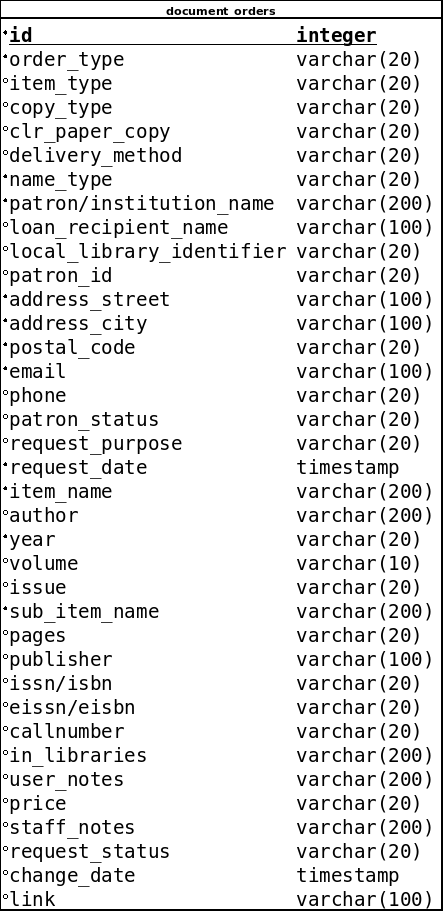
\includegraphics[width=0.65\textwidth]{tlacitko}
\centering
\caption{N�vrh rela�n� datab�ze pro spr�vu objedn�vek dokument�. Autorem je Daniel Mare�ek.}
\label{fig:tlacitko}
\end{figure}

Mezi dal�� tuzemsk� instituce s vyhled�va�em VuFind pat�� M�stsk� knihovna �esk� T�ebov�, jej� instalace verze VuFind 2.3 v prost�ed� linuxov� distribuce opera�n�ho syst�mu Debian je propojena s integrovan�m knihovnick�m syst�mem Koha.
M�stsk� knihovna �st� nad Orlic� provozuje VuFind 2.4.1 tak� v linuxov� distribuci opera�n�ho syst�mu Debian s napojen�m na integrovan� knihovnick� syst�m Koha. Grafick� vzhled katalog� obou knihoven vych�z� ze standardu Bootstrap3.

Souborn� katalog Akademie v�d �R pro webov� rozhran� tak� pou��v� VuFind a to verzi z �ady 1.x. Zde je mo�no prohled�vat ve v�ech �stavech najednou, nebo tak� v ka�d�m �stavu samostatn�, co� znamen�, �e pro ka�d� �stav existuje odd�len� index. V t�to instalaci je nastaveno pou�it� technologie OpenSearch.
\cite{avcr}

V �esk� republice lze nal�zt u�ivatelsk� rozhran� VuFind i v komer�n�m projektu, kter� nab�z� integrovan� knihovnick� syst�m Koha jako slu�bu (SystemAsAService). T�mto zp�sobem pou��v� port�l VuFind knihovna v Poli�ce, Turnov�, Neratovic�ch, Jablonci nad Nisou a Fren�t�t�. \cite{koha.vufind}


Zaj�mav� p��pad, kdy se po testov�n� port�lu VuFind rozhodlo pro v�b�r jin�ho �e�en�, se odehr�l v americk� univerzitn� knihovn� Yale University Library. N�jak� �as testov�n� prob�halo pod pracovn�m n�zvem YuFind, ale k pou�it� v ostr�m provozu nedo�lo. \cite{yale}



\chapter{Budouc� v�voj syst�mu}
\label{sec:chapter05}
Rozd�l oproti integrovan�m knihovnick�m syst�m�m, kter� poskytuj� ve�ejn� on-line rozhran� katalogu, je v tom, �e projekt VuFind se zam��uje v�hradn� na u�ivatelsk� rozhran� a na integraci s ostatn�mi knihovn�mi slu�bami. Proto m� obrovsk� potenci�l zast�e�it v�ce vyhled�vac�ch slu�eb pod jeden sjednocen� interface. Krom� toho, �e VuFind m� pojmout v�ce integrovan�ch knihovnick�ch syst�mu a datab�z� elektronick�ch informa�n�ch zdroj�, mus� se vypo��dat se st�le rostouc� pot�ebou rozli�ovat licen�n� pr�va pro p��stup do sv�tov�ch datab�zov�ch zdroj� pro v�ce skupin u�ivatel�. Toto je po�adavek p�edev��m knihoven, kter� integruj� men�� okoln� knihovny. P��kladem je NTK, kde se tato problematika �e��. D�ky st�le rostouc� komunit�, a� u� v�voj��� nebo u�ivatel� VuFindu, se tento nedostatek m��e do budoucna vy�e�it ve st�le p��v�tiv�m v�vojov�m prost�ed� PHP.

V kv�tnu roku 2016 vy�la nov� verze port�lu VuFind 3.0, kter� pou��v� novou verzi indexa�n�ho n�stroje Solr a p�in�� mnoh� dal�� vylep�en� \cite{changelog}. Ve�ejn� on-line katalog NTK na tuto verzi p�ejde, potom co bude verze implementov�na a otestov�na v lok�ln�ch podm�nk�ch. Dal�� v�zvou pro NTK je uv�st do provozu syst�m VuFind s napojen�m discovery slu�by Summon, je� je v tuto chv�li v experiment�ln� f�zi.

Mo�n� by snad mohlo b�t i uva�ovat o nahrazen� komer�n�ho integrovan�ho knihovnick�ho syst�mu Aleph svobodnou alternativou syst�mem Koha v NTK.


\chapter{Z�v�r (zhodnocen�)}
\label{sec:conclusion}
ڞasn�, super, m� budoucnost, mohlo by b�t dobr�m byznysem nasazovat VuFind do dal��ch knihoven - po cel�m sv�t�. 4-let� pr�ce s velk�m p��nosem zku�enost� z praxe v oboru. ��ast na zaj�mav�ch konferenc�ch - Inforum, Elag, KRE,. 

\medskip

\begin{thebibliography}{9}
\bibitem{techlib} 
O NTK: V� partner ve sv�t� technick�ch informac�. \textit{N�rodn� technick� knihovna} [online]. Praha [cit. 2016-06-09]. Dostupn� z: https://www.techlib.cz/cs/82794-o-ntk

\bibitem{stk} 
\textit{St�tn� technick� knihovna} [online]. Praha [cit. 2016-06-09]. Dostupn� z: http://old.stk.cz/index.html

\bibitem{vufind.org} 
Installation:fedora [VuFind Documentation]. VuFind - Search. Discover. Share. [online]. [cit. 2016-06-10]. Dostupn� z: https://vufind.org/wiki/installation:fedora
\end{thebibliography}

\appendix
\chapter{P��loha}
\input{chapters/appendix}

\end{document}
